\section{Chapter 3: Labor Demand}

\subsection{Terms}

\begin{itemize}
    \item $q$: Quantity of output produced by the firm
    \item $E$: Employee-hours (labor input)
    \item $K$: Capital input (machines, land, etc.)
    \item $MP_E$: Marginal product of labor
    \item $MP_K$: Marginal product of capital
    \item $p$: Price of output
    \item $w$: Wage rate (price of labor)
    \item $r$: Rental rate (price of capital)
    \item $VMP_E$: Value of marginal product of labor
    \item $VAP_E$: Value of average product of labor
    \item $C$: Cost of production
\end{itemize}

\subsection{The Firm's Production Function}

The firm's production function 
describes the technology that the firm 
uses to produce its output.
We will assume for the moment that 
the firm only requires two inputs for 
its production: labor in the form of 
employee-hours ($E$) and capital ($K$),
which includes land, machines, 
and other physical inputs.
We will write the firm's production function as:

\begin{align}
    q=f(E, K)
\end{align}

%%%%%%%%%%%%%%%%%%%%%%%%%%%%%%%%%%%%%%%%%%%%%%%%%%%%%%%%%%%%%%%%%%%%%%%%%%%%%%%%%%%%%%%
\subsubsection{Marginal Product and Average Product}

\begin{definition}[Marginal Product of Labor] 
    
    The marginal product of labor ($MP_E$)
    is the additional output produced
    as a result of hiring one more
    employee-hour, holding the amount
    of capital constant.

\end{definition}

\begin{definition}[Marginal Product of Capital]

    The marginal product of capital ($MP_K$)
    is the additional output produced
    as a result of using one more
    unit of capital, holding the amount
    of labor constant.

\end{definition}

\begin{definition}[Average Product of Labor]

    The average product of labor ($AP_E$)
    is the average output produced per employee-hour,
    holding the amount of capital constant.

    \begin{align}
        AP_E = \frac{q}{E}
    \end{align}
    
\end{definition}

\begin{definition}[Law of Diminishing Returns] 
    
    This is the assumption that the marginal 
    product of labor eventually declines.

\end{definition}


\autoref{fig:ch_3p1_marg_prod_table}
shows an example of how we would calculate 
the marginal product, average product, value of 
marginal product, and value of average product for labor.

\FloatBarrier

\begin{figure}[!htb]
    \centering
        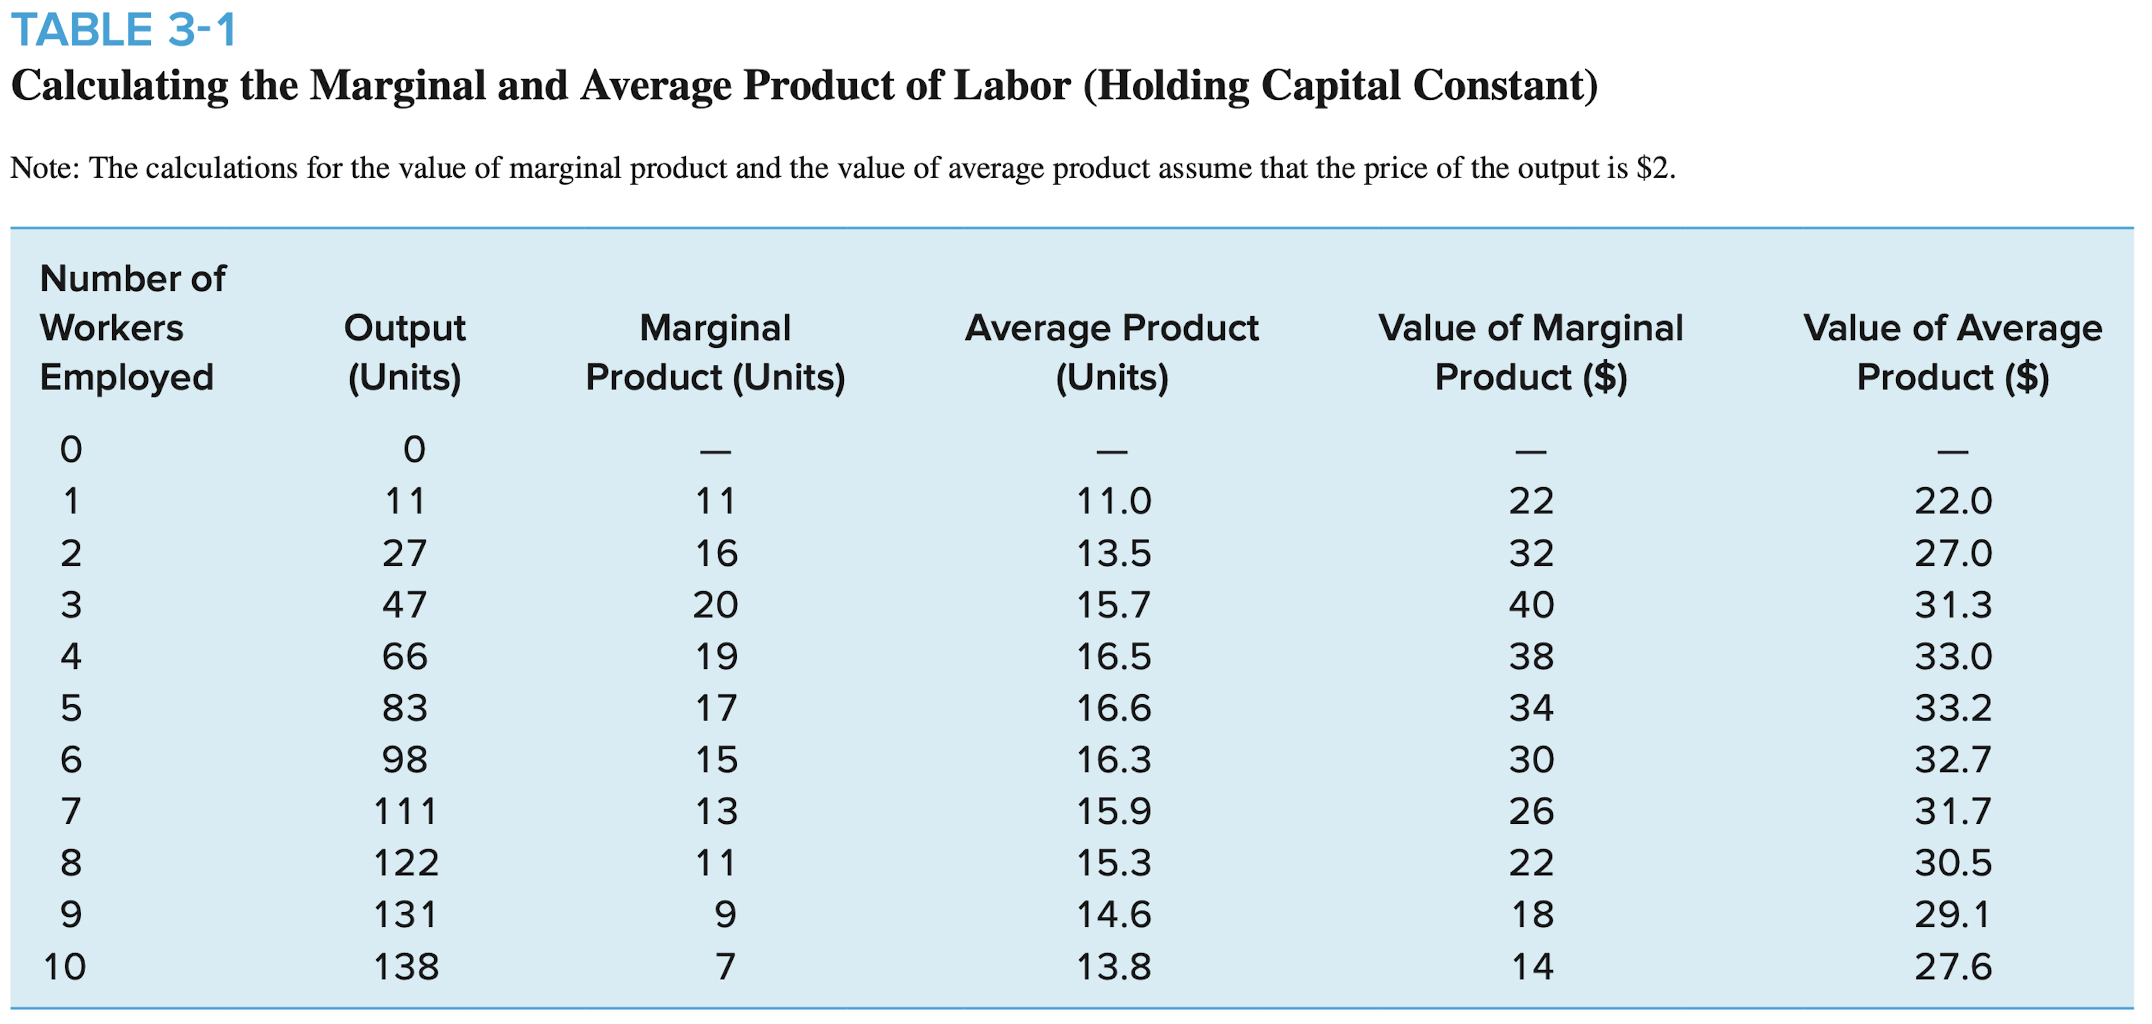
\includegraphics[width=0.95\textwidth]{../input/ch_3p1_marg_prod_table.png}
    \caption{Marginal Product Table}
    \label{fig:ch_3p1_marg_prod_table}
\end{figure}

\FloatBarrier

\autoref{fig:ch_3p1_marg_prod_av_prod}
shows the relationship between the marginal product
and average product curves.

\FloatBarrier

\begin{figure}[!htb]
    \centering
        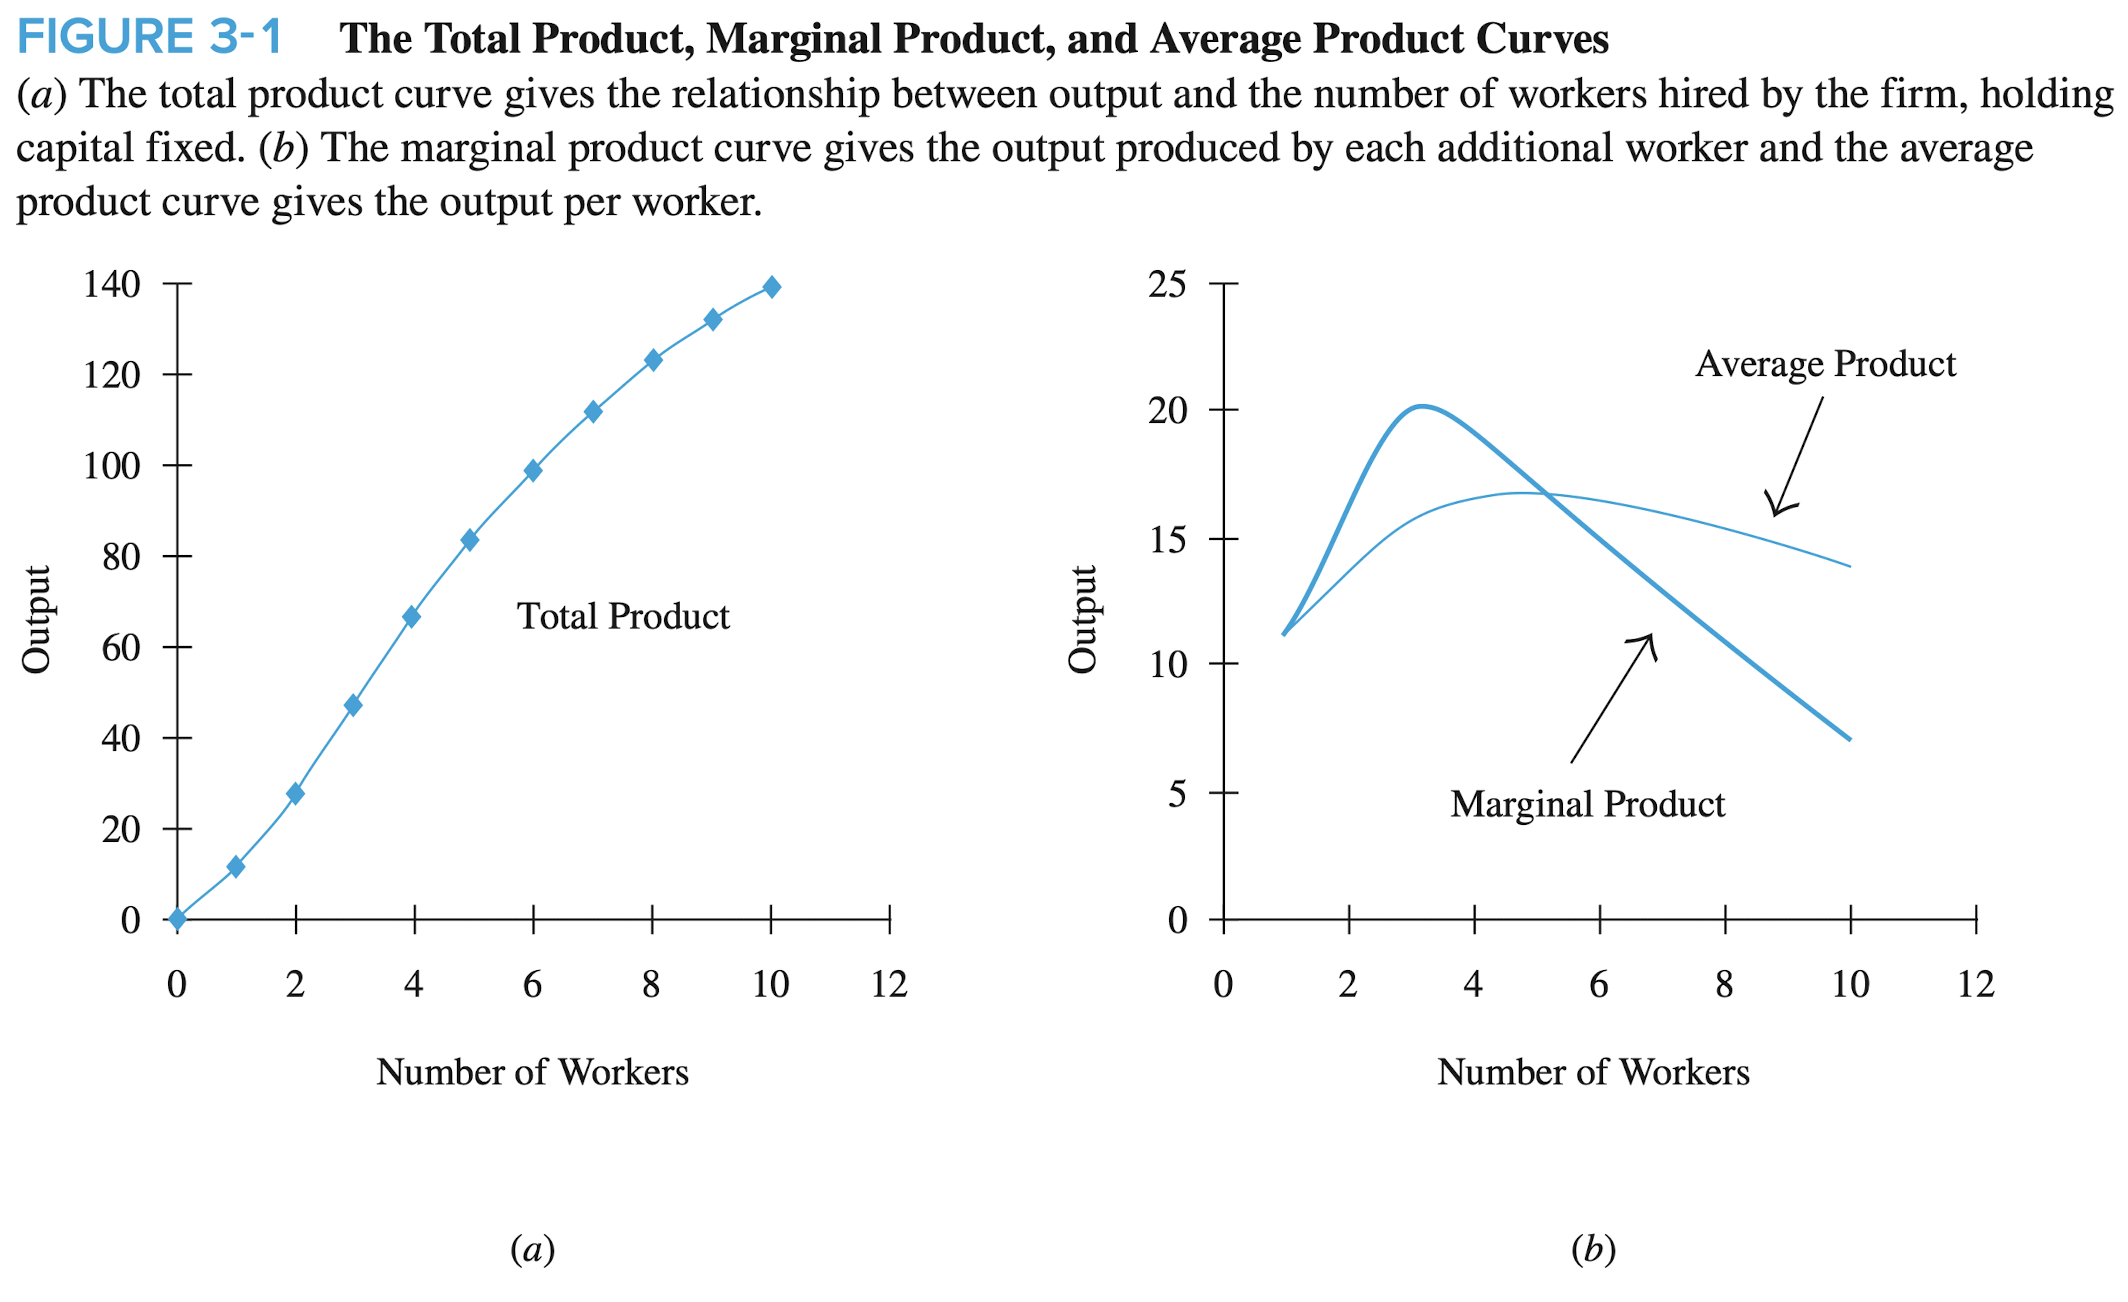
\includegraphics[width=0.9\textwidth]{../input/ch_3p1_marg_prod_av_prod.png}
    \caption{Marginal Product and Average Product Curves}
    \label{fig:ch_3p1_marg_prod_av_prod}
\end{figure}

\FloatBarrier

%%%%%%%%%%%%%%%%%%%%%%%%%%%%%%%%%%%%%%%%%%%%%%%%%%%%%%%%%%%%%%%%%%%%%%%%%%%%%%%%%%%%%%%
\subsubsection{Profit Maximization}


The firm's profits are given by

\begin{align}
    \text{Profits} &= p q - w E - r K
\end{align}

where 

\begin{itemize}
    \item $p$: Price of output
    \item $w$: Wage rate (price of labor)
    \item $r$: Rental rate (price of capital)
\end{itemize}

We assume that the firm is maximizing profits.
We also, for the moment, take firms to be 
perfectly competitive, i.e., they cannot influence prices. 
Thus, given that these firms are price takers,
they will maximize profits by 
choosing the optimal quantity of labor 
and capital.

\begin{definition}[Perfectly Competitive Firm]

    We refer to a perfectly competitive firm as 
    one that cannot influence prices. 

\end{definition}

%%%%%%%%%%%%%%%%%%%%%%%%%%%%%%%%%%%%%%%%%%%%%%%%%%%%%%%%%%%%%%%%%%%%%%%%%%%%%%%%%%%%%%%
%%%%%%%%%%%%%%%%%%%%%%%%%%%%%%%%%%%%%%%%%%%%%%%%%%%%%%%%%%%%%%%%%%%%%%%%%%%%%%%%%%%%%%%
\subsection{The Short Run}

\begin{definition}[The Short Run] 
    
    In our context, we define the short run to be a time horizon
    that is sufficiently short such that the firm 
    cannot adjust its capital stock ($K$).

\end{definition}

\begin{definition}[Value of Marginal Product of Labor] 

    The value of the marginal product of labor ($VMP_E$)
    is the additional revenue generated
    as a result of hiring one more
    employee-hour, holding the amount
    of capital constant.

    \begin{align}
        VMP_E = p \cdot MP_E
    \end{align}
    
\end{definition}

\begin{definition}[Value of Average Product of Labor]
    
    The value of the average product of labor ($VAP_E$)
    is the average revenue generated per employee-hour,
    holding the amount of capital constant.

    \begin{align}
        VAP_E = p \cdot AP_E
    \end{align}
    
\end{definition}

%%%%%%%%%%%%%%%%%%%%%%%%%%%%%%%%%%%%%%%%%%%%%%%%%%%%%%%%%%%%%%%%%%%%%%%%%%%%%%%%%%%%%%%
\subsubsection{How Many Workers Should the Firm Hire?}

The firm will hire workers up to the point that 
the value of the marginal product of labor 
equals the wage rate and the value of the marginal product 
of labor is downward sloping. See 
\autoref{fig:ch_3p2_short_run_hiring}
for an example of $VMP_E$ and $VAP_E$ curves.
In this figure, see the horizontal lines at 
$22$ and $38$. If the wage rate is $22$,
then the firm will hire $8$ employees.\footnote{I think I'm kind 
of using employees and employee-hours as interchangeable concepts
here.}
If the wage rate is $38$, then the firm will
hire $4$ employees.


\FloatBarrier

\begin{figure}[!htb]
    \centering
        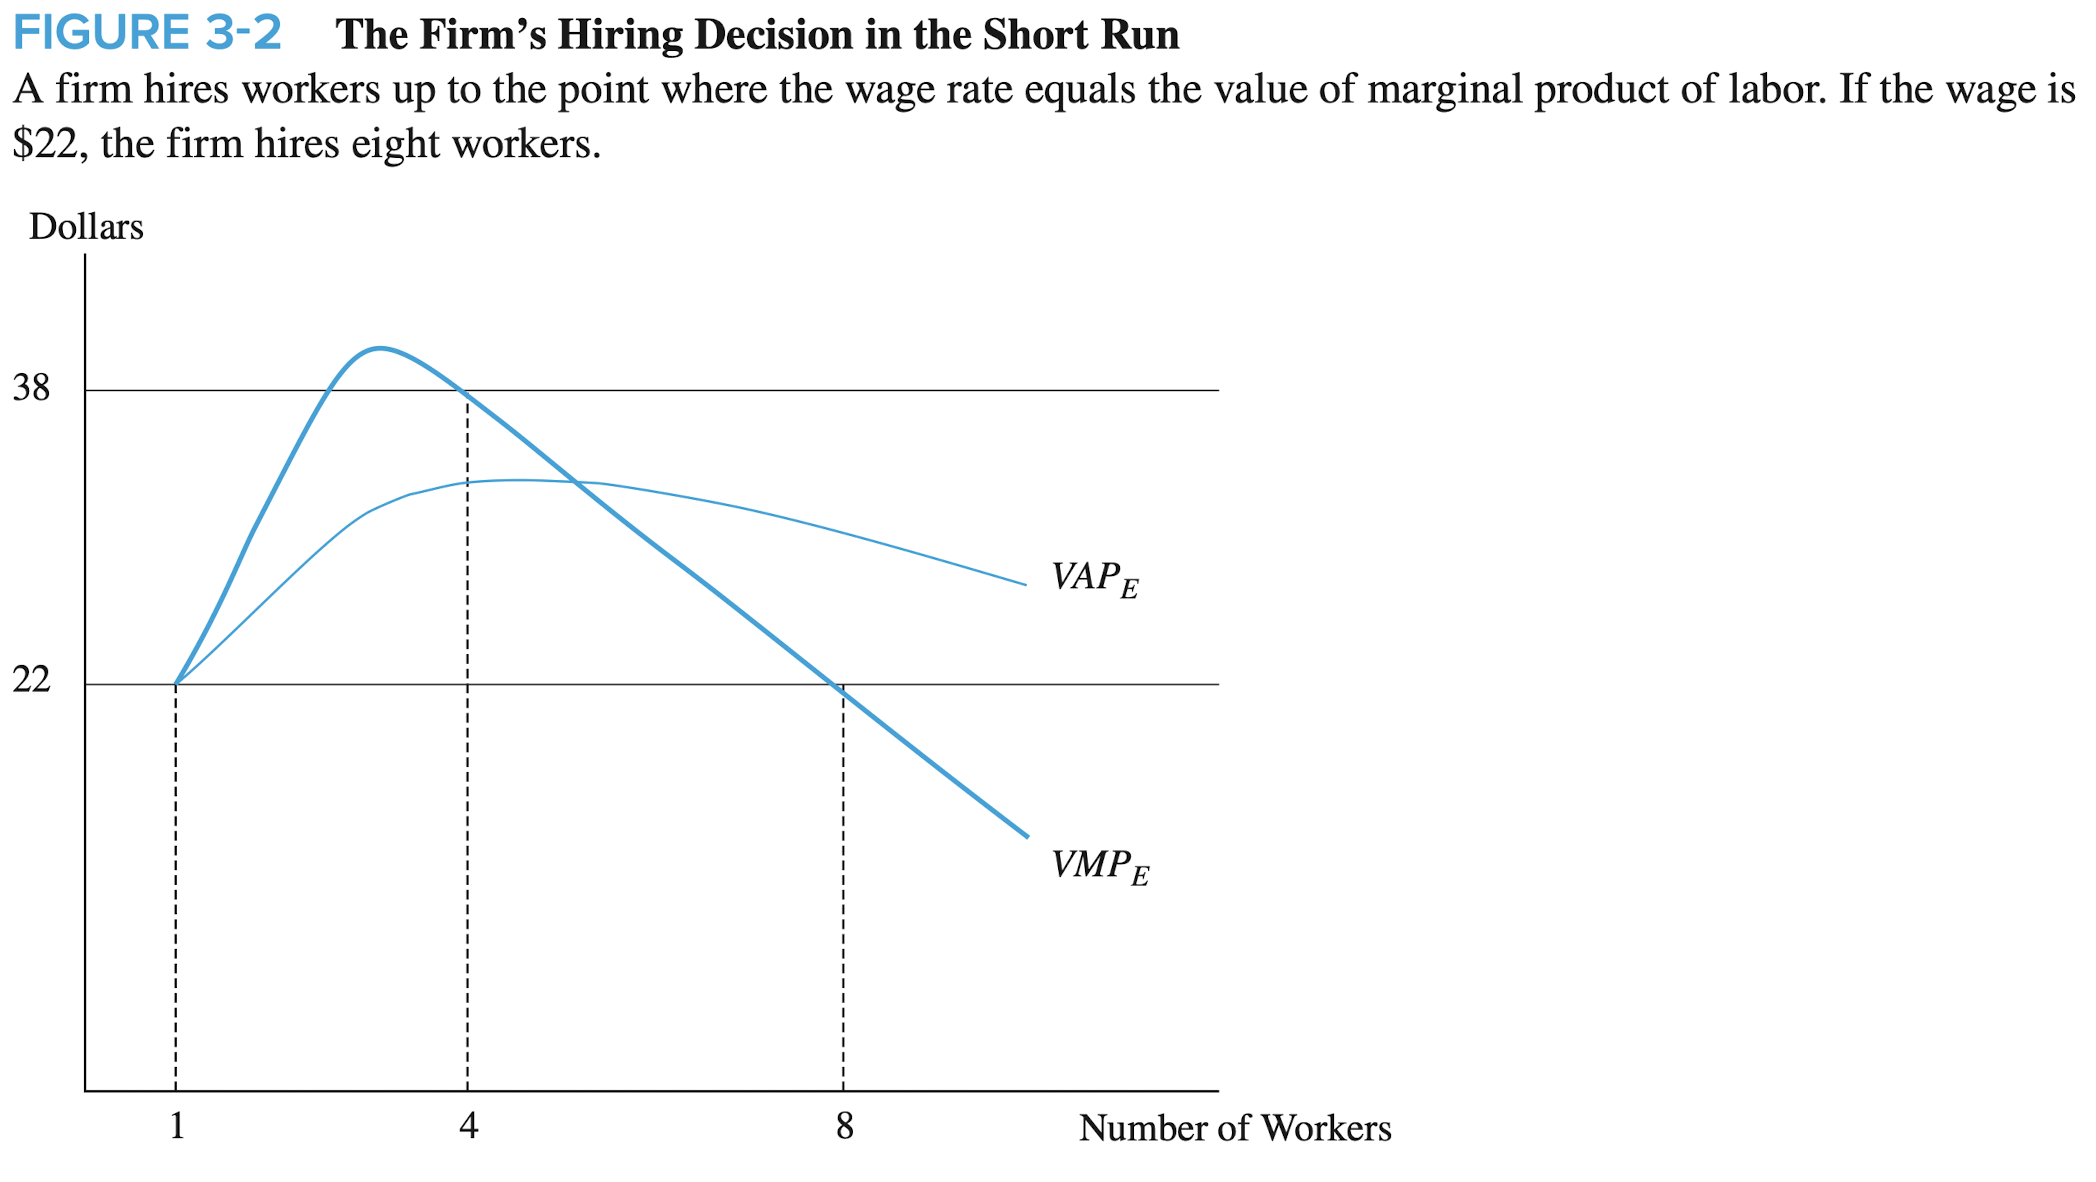
\includegraphics[width=0.9\textwidth]{../input/ch_3p2_short_run_hiring.png}
    \caption{Short Run Hiring Decision}
    \label{fig:ch_3p2_short_run_hiring}
\end{figure}

\FloatBarrier

%%%%%%%%%%%%%%%%%%%%%%%%%%%%%%%%%%%%%%%%%%%%%%%%%%%%%%%%%%%%%%%%%%%%%%%%%%%%%%%%%%%%%%%
\subsubsection{The Short-Run Labor Demand Curve for a Firm}

With this setup, we can now derive the 
firm's short-run labor demand curve. 
In particular, 
the short-run labor-demand curve is given by
the value of the marginal product of labor curve.
In particular, we can look at \autoref{fig:ch_3p2_short_run_hiring},
see at each value on the $y$-axis as a potential wage, 
draw a horizontal line to the
point on the $VMP_E$ curve that it intersects and is downward sloping,
and then drop down to the $x$-axis to see how many employees
the firm would hire at that wage.
Doing this for all potential wages gives us the
short-run labor demand curve, which is shown in
\autoref{fig:ch_3p2_short_run_labor_demand}.
\autoref{fig:ch_3p2_short_run_labor_demand}
also depicts what would happen if there was a shift 
in the $VMP_E$ curve stemming from a 
rise in the price of the output. This would 
lead to more workers being hired, since it would 
raise the $VMP_E$ curve to $VMP_{E'}$.


\FloatBarrier

\begin{figure}[!htb]
    \centering
        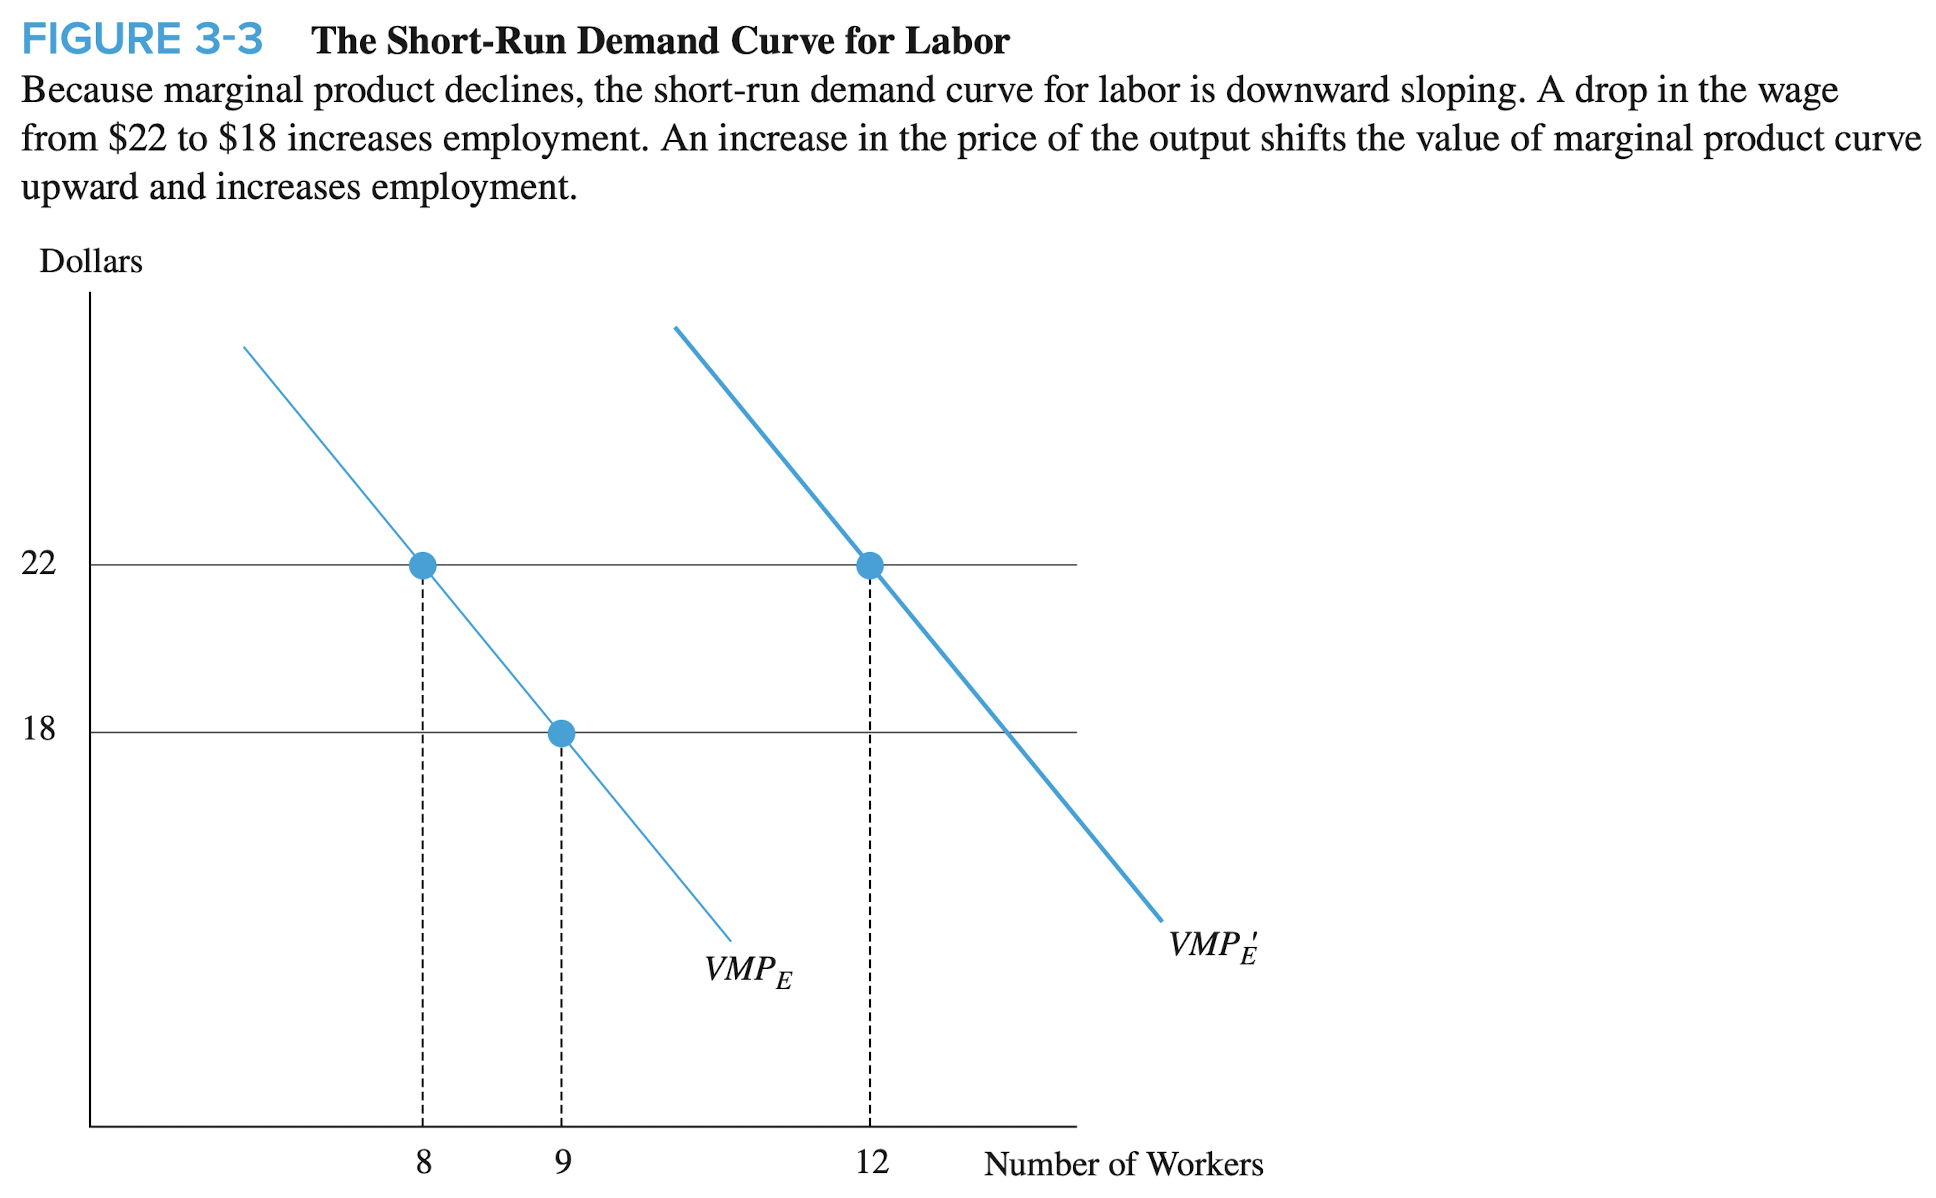
\includegraphics[width=0.9\textwidth]{../input/ch_3p2_short_run_labor_demand.png}
    \caption{Short-Run Labor Demand Curve}
    \label{fig:ch_3p2_short_run_labor_demand}
\end{figure}

\FloatBarrier

\begin{overview}[Critical Point]
    
    It will be a recurring point to remember that 
    the short-run labor demand curve for a firm
    is given by the $VMP_E$ curve.

\end{overview}

%%%%%%%%%%%%%%%%%%%%%%%%%%%%%%%%%%%%%%%%%%%%%%%%%%%%%%%%%%%%%%%%%%%%%%%%%%%%%%%%%%%%%%%
\subsubsection{The Short-Run Labor Demand Curve in the Industry}

The short-run labor demand curve in the industry 
is not simply the sum of the short-run labor demand curves
of the individual firms, because, while one firm 
cannot influence prices, the industry as a whole can.
If the industry increases production dramatically,
the price of the output will fall, which lowers
the $VMP_E$ curve and hence demand. 
Thus, the short-run labor demand curve in the industry
reflects this. See 
\autoref{fig:ch_3p2_short_run_industry_demand}
for an illustration.

\FloatBarrier

\begin{figure}[!htb]
    \centering
        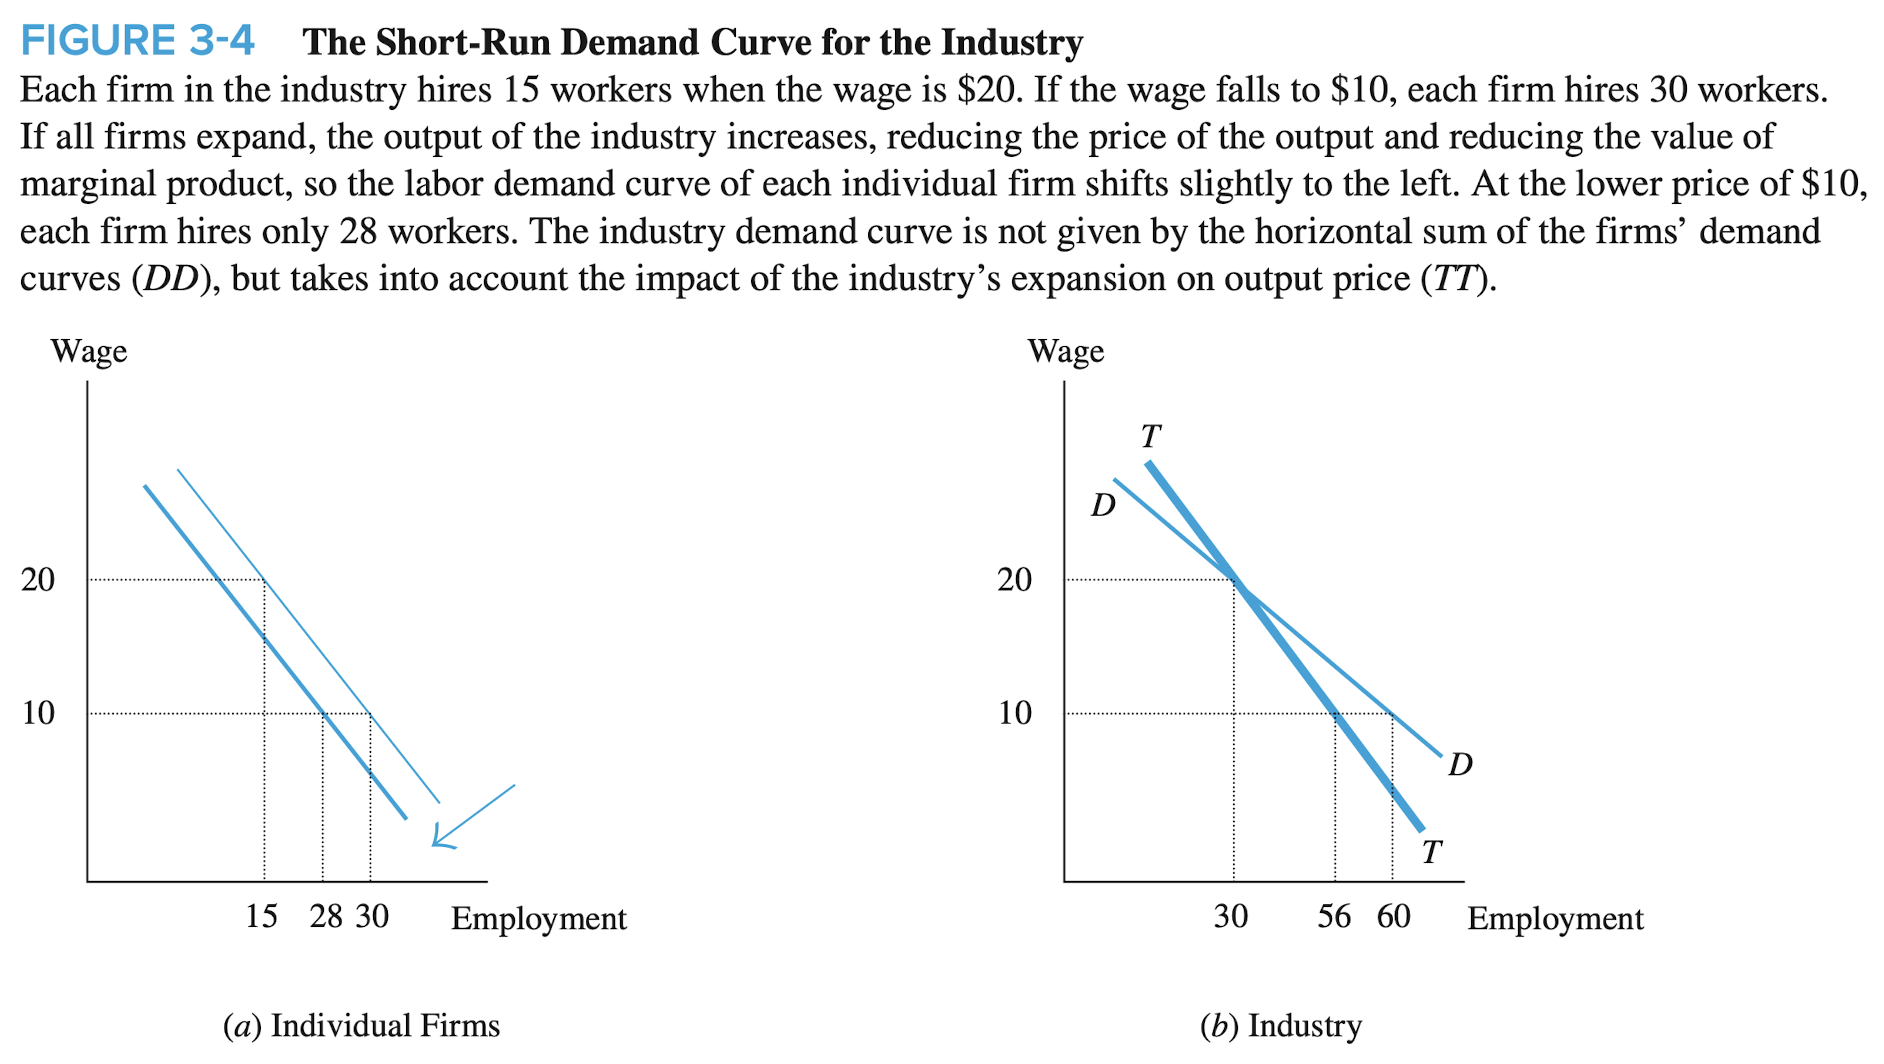
\includegraphics[width=0.9\textwidth]{../input/ch_3p2_short_run_industry_demand.png}
    \caption{Short-Run Labor Demand Curve in the Industry}
    \label{fig:ch_3p2_short_run_industry_demand}
\end{figure}

\FloatBarrier

\begin{definition}[Elasticity of Labor Demand]

    The elasticity of labor demand ($\delta_{SR}$)
    is the percentage change in the quantity of labor demanded in the 
    short run ($E_{SR}$)
    resulting from a percentage change in the wage rate.
    
    \begin{align}
        \delta_{S R}=\frac{\Delta E_{S R} / E_{S R}}{\Delta w / w}=\frac{\Delta E_{S R}}{\Delta w} \cdot \frac{w}{E_{S R}}
    \end{align}
    
\end{definition}

%%%%%%%%%%%%%%%%%%%%%%%%%%%%%%%%%%%%%%%%%%%%%%%%%%%%%%%%%%%%%%%%%%%%%%%%%%%%%%%%%%%%%%%
\subsubsection{An Alternative Interpretation of the Marginal Productivity Condition}

An alternative way to express the point that the 
firm hires up to the point that the 
value of the marginal product of labor equals the wage rate is the following: 
The firm will hire up to the point that its marginal 
cost (MC)\footnote{That is, the marginal cost of 
producing another unit of the output.} equals its marginal revenue (MR).
This interpretation is illustrated in 
\autoref{fig:ch_3p2_mc_firm_output}, where 
we show the marginal cost curve intersecting 
the marginal revenue curve (which in this case, 
is simply the price of the output, $p$).
The optimal quantity of output is then 
given by $q^*$.

\FloatBarrier

\begin{figure}[!htb]
    \centering
        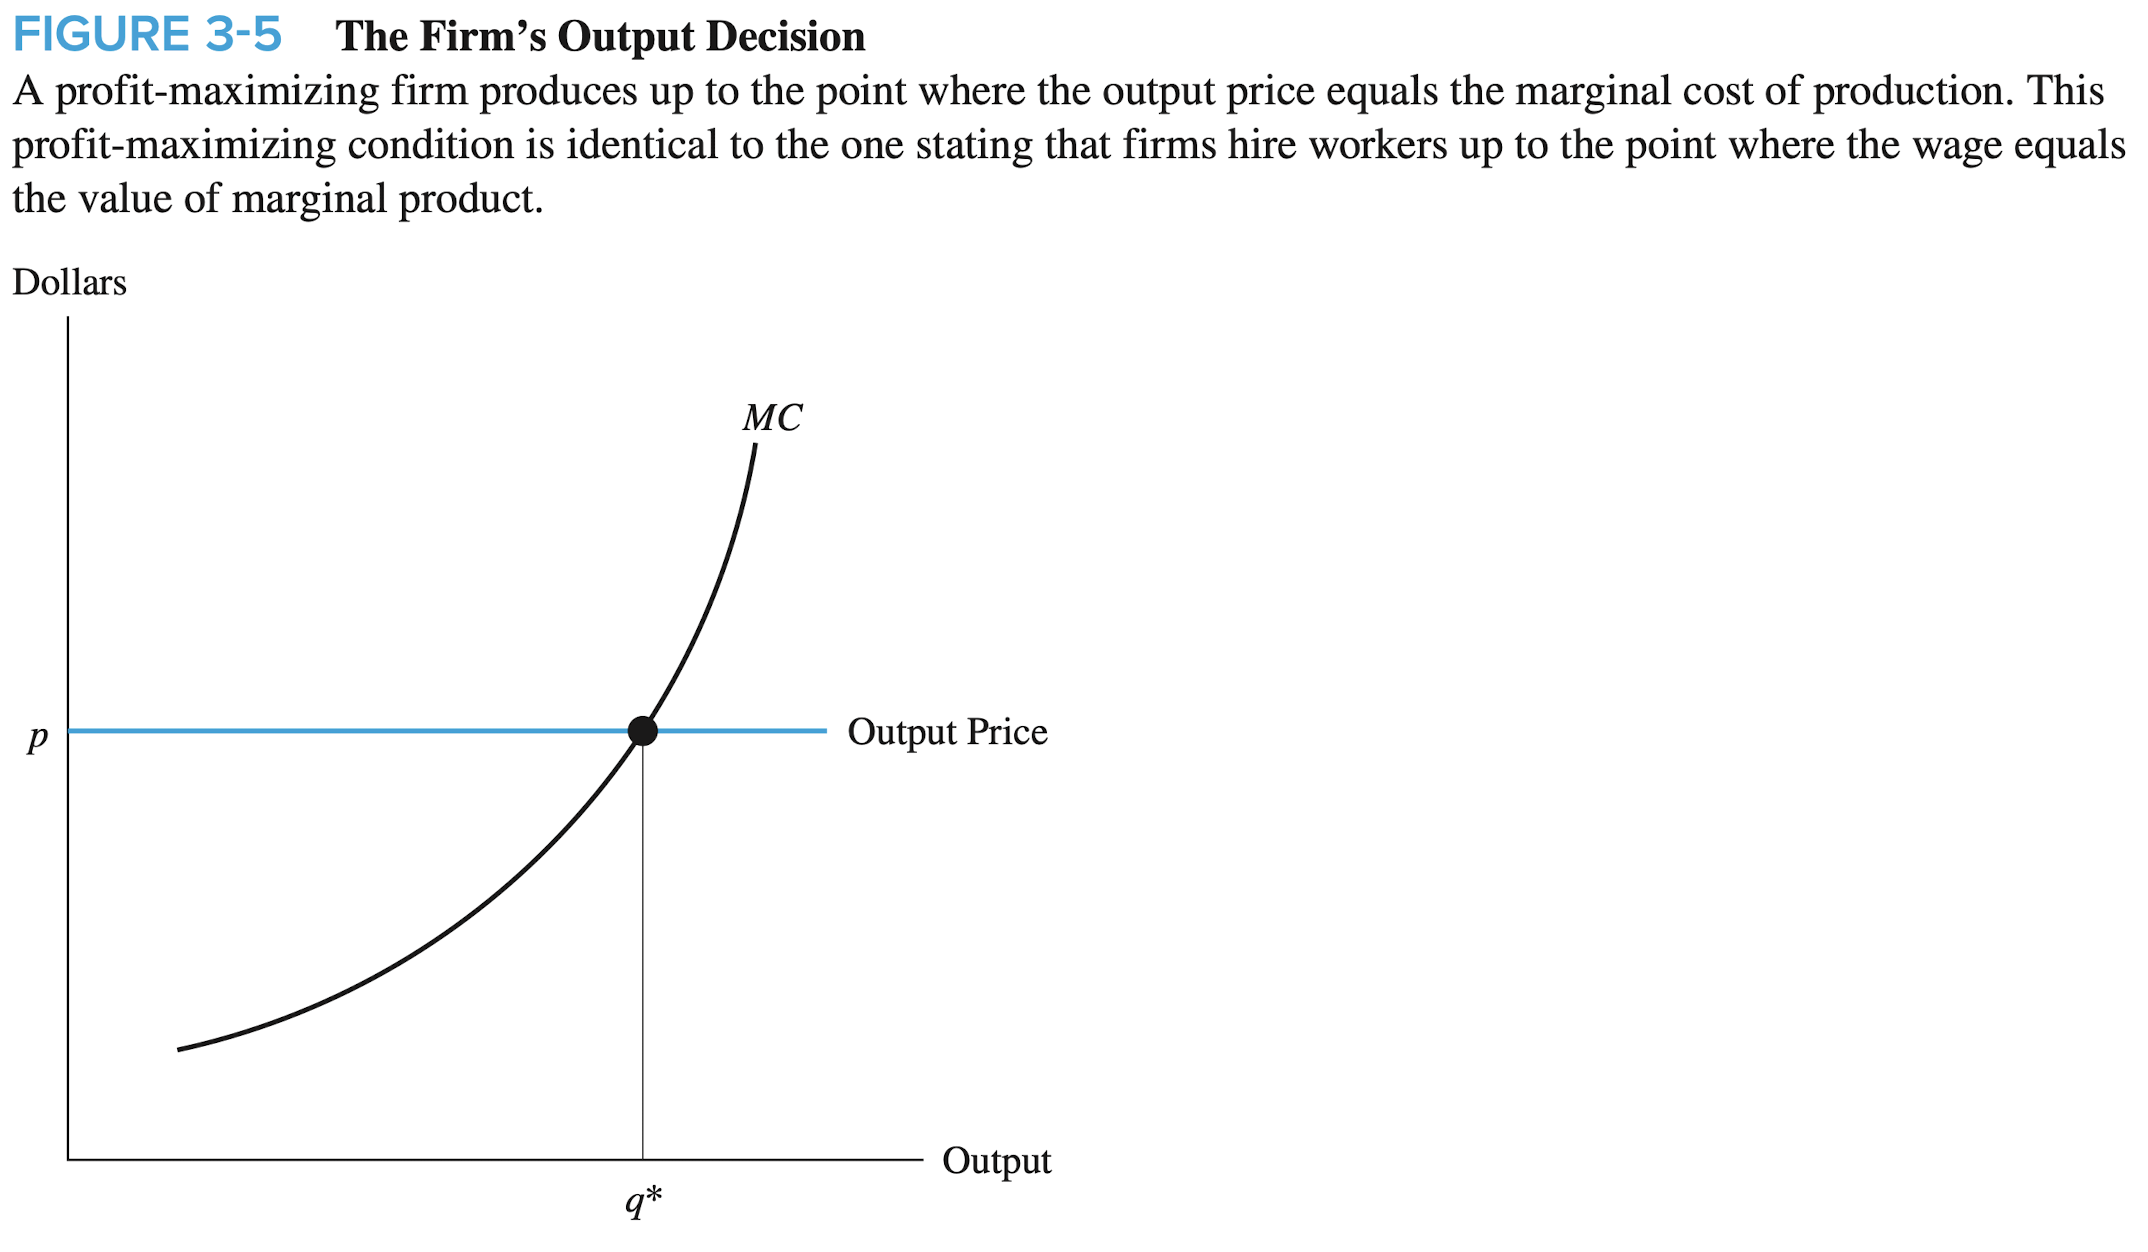
\includegraphics[width=0.9\textwidth]{../input/ch_3p2_mc_firm_output.png}
    \caption{The Firm's Output Decision}
    \label{fig:ch_3p2_mc_firm_output}
\end{figure}

\FloatBarrier

We can note that the 
marginal cost of 
producing an extra unit of output is given by:

\begin{align}
    M C=w \times \frac{1}{M P_E}
\end{align}

That is, the wage scaled down by 
the marginal product of labor.\footnote{You can think of 
this as saying something like: How much of a worker would you 
need to produce one more unit of output?}

Then, the profit-maximizing 
condition is that

\begin{align}
    &w \times \frac{1}{M P_E}=p \\
    \text{or } &w=p \times M P_E = V M P_E
\end{align}

%%%%%%%%%%%%%%%%%%%%%%%%%%%%%%%%%%%%%%%%%%%%%%%%%%%%%%%%%%%%%%%%%%%%%%%%%%%%%%%%%%%%%%%
%%%%%%%%%%%%%%%%%%%%%%%%%%%%%%%%%%%%%%%%%%%%%%%%%%%%%%%%%%%%%%%%%%%%%%%%%%%%%%%%%%%%%%%
\subsection{The Long Run}

\subsubsection{Isoquants}

\begin{definition}[Isoquant] 
    
    An isoquant is a curve that captures the 
    different combinations of labor and capital
    that produce the same level of output.

\end{definition}

We demand the following properties of isoquants:

\begin{enumerate}
    \item Isoquants must be downward sloping.
    \item Isoquants do not intersect.
    \item Higher isoquants are associated with higher levels of output.
    \item Isoquants are convex to the origin.
\end{enumerate}

See \autoref{fig:ch_3p3_isoquant_intro}
for an illustration of isoquants.
Notice, as one would expect based on the 
definition, we are 
plotting the isoquants in $K$-$E$ space.

\FloatBarrier

\begin{figure}[!htb]
    \centering
        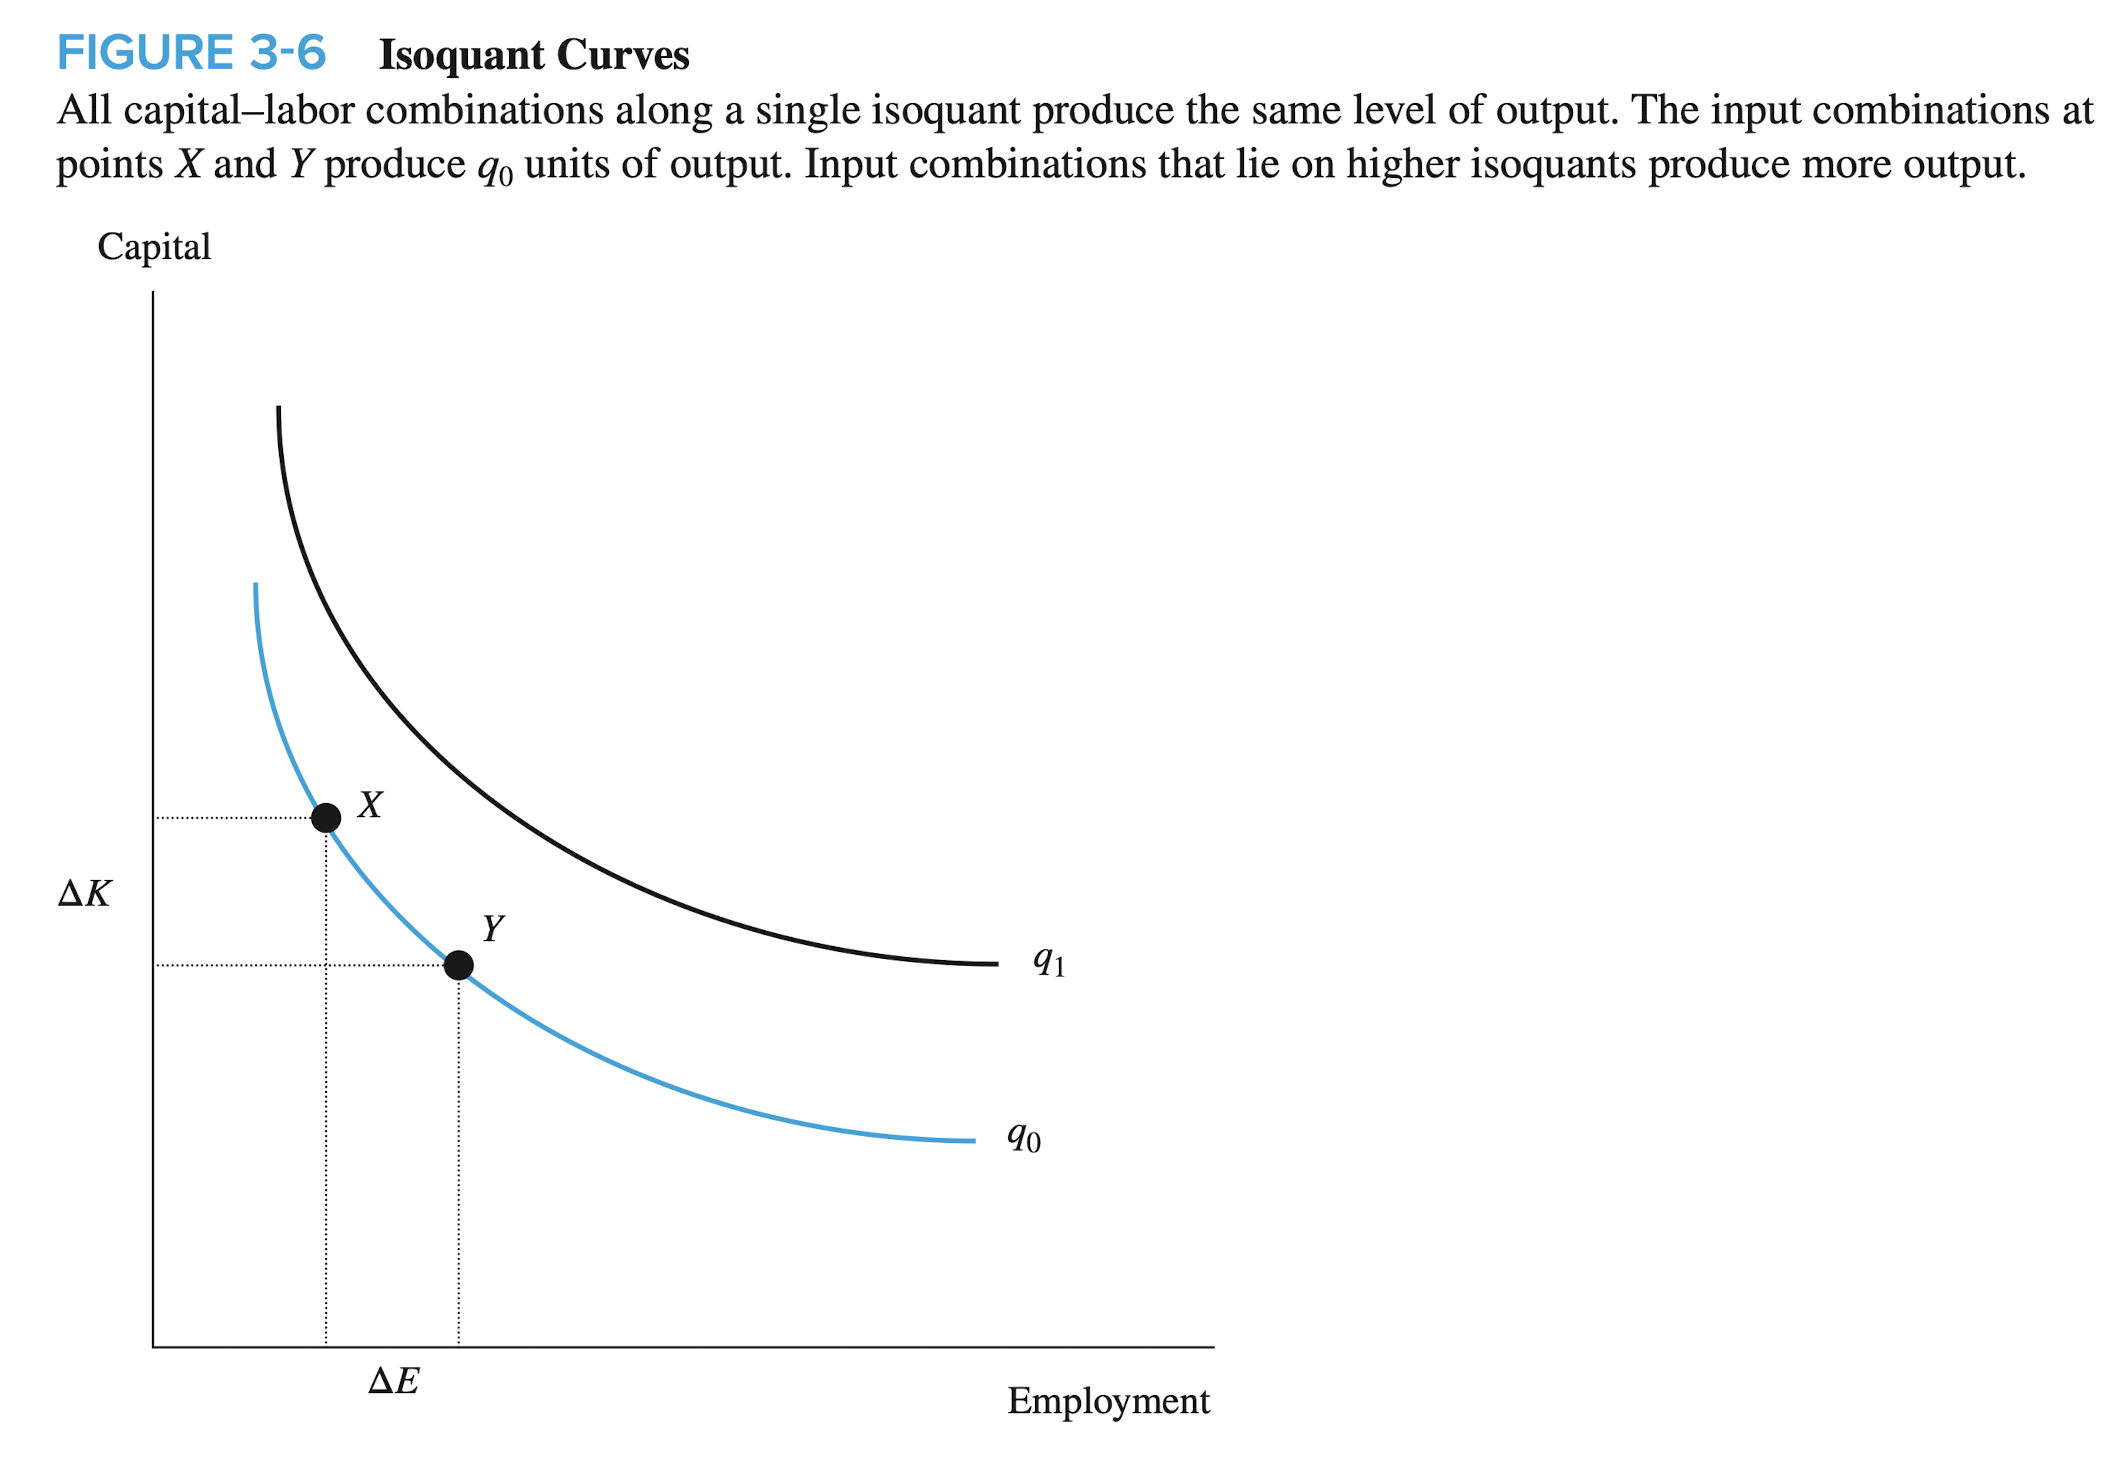
\includegraphics[width=0.95\textwidth]{../input/ch_3p3_isoquant_intro.png}
    \caption{Isoquant Illustration}
    \label{fig:ch_3p3_isoquant_intro}
\end{figure}

\FloatBarrier

The slope of the isoquant is given by 

\begin{align}
    \frac{\Delta K}{\Delta E}=-\frac{M P_E}{M P_K}
\end{align}

The LHS just captures the standard rise-over-run 
definition of slope. The RHS stems from the fact that,
given the definition of an isoquant,
it must be that:

\begin{align}
    (\Delta K) MP_K + (\Delta E) MP_E = 0
\end{align}

Thus, the slope of the isoquant is the 
negative ratio of the marginal products.

\begin{definition}[Marginal Rate of Technical Substitution]
    
    The absolute value of the slope of the 
    isoquant is referred to as the marginal rate of technical substitution (MRTS).
    That is, the MRTS is given by:

    \begin{align}
        MRTS = \left| \frac{\Delta K}{\Delta E} \right| = \frac{M P_E}{M P_K}
    \end{align}

    Intuitively, this is telling us, if we increase labor by one unit, 
    how much capital can we give up, while still keeping output constant.\footnote{
        The ``one unit'' framing isn't really right, since it's 
        really about infinitesimal changes, but
        I'm being a little loose for the intuition.
    }
    
\end{definition}

%%%%%%%%%%%%%%%%%%%%%%%%%%%%%%%%%%%%%%%%%%%%%%%%%%%%%%%%%%%%%%%%%%%%%%%%%%%%%%%%%%%%%%%
\subsubsection{Isocosts}

The firm's cost of production is given by:

\begin{align}
    C=w E+r K
\end{align}

\begin{definition}[Isocost Line] 
    
    An isocost line is a curve that captures the 
    different combinations of labor and capital
    that yield the same cost of production.

\end{definition}

See \autoref{fig:ch_3p3_isocost_intro}
for an illustration of isocost lines.

\FloatBarrier

\begin{figure}[!htb]
    \centering
        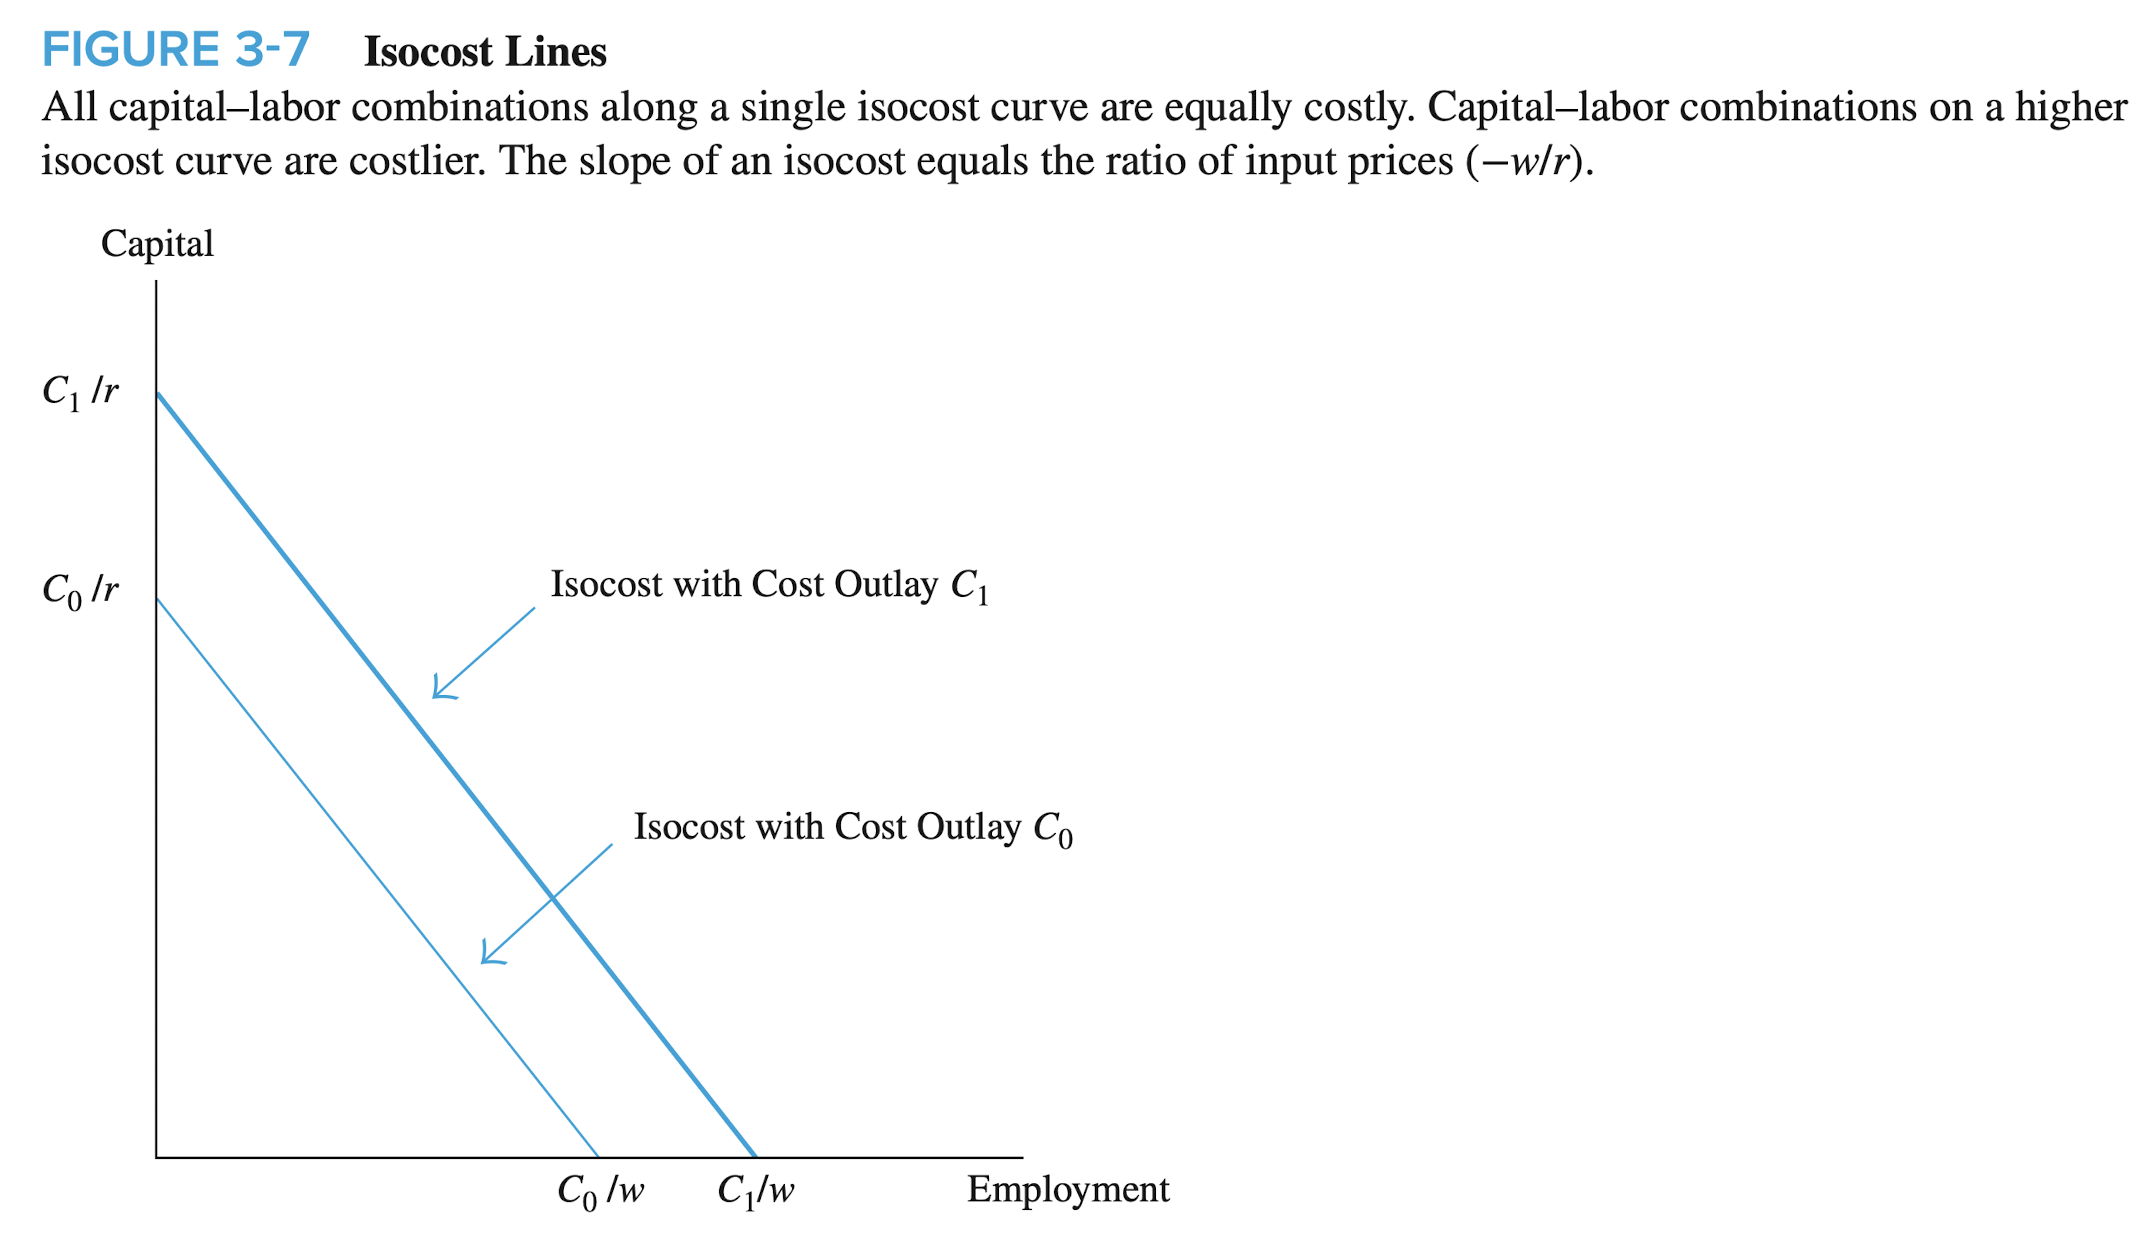
\includegraphics[width=0.95\textwidth]{../input/ch_3p3_isocost_intro.png}
    \caption{Isocost Lines}
    \label{fig:ch_3p3_isocost_intro}
\end{figure}

\FloatBarrier

We can re-write the isocost line 
as:

\begin{align}
    K=\frac{C}{r}-\frac{w}{r} E
\end{align}

Thus, we can see that the slope of the isocost line 
is given by: $-\frac{w}{r}$.
This is intuitive since it's telling us that 
the slope corresponds to telling us that 
an additional unit of labor costs 
$\frac{w}{r}$ units of capital.

%%%%%%%%%%%%%%%%%%%%%%%%%%%%%%%%%%%%%%%%%%%%%%%%%%%%%%%%%%%%%%%%%%%%%%%%%%%%%%%%%%%%%%%
\subsubsection{Cost Minimization}

Suppose that the firm is going to 
produce $q_0$ units of output. 
We can then ask: how can the firm
produce $q_0$ at the lowest cost?
The solution to this question is illustrated 
in \autoref{fig:ch_3p3_cost_min}.
The cost-minimizing solution is to 
produce at the point along the isocost line 
for $q_0$ which has a tangent isoquant.

\FloatBarrier

\begin{figure}[!htb]
    \centering
        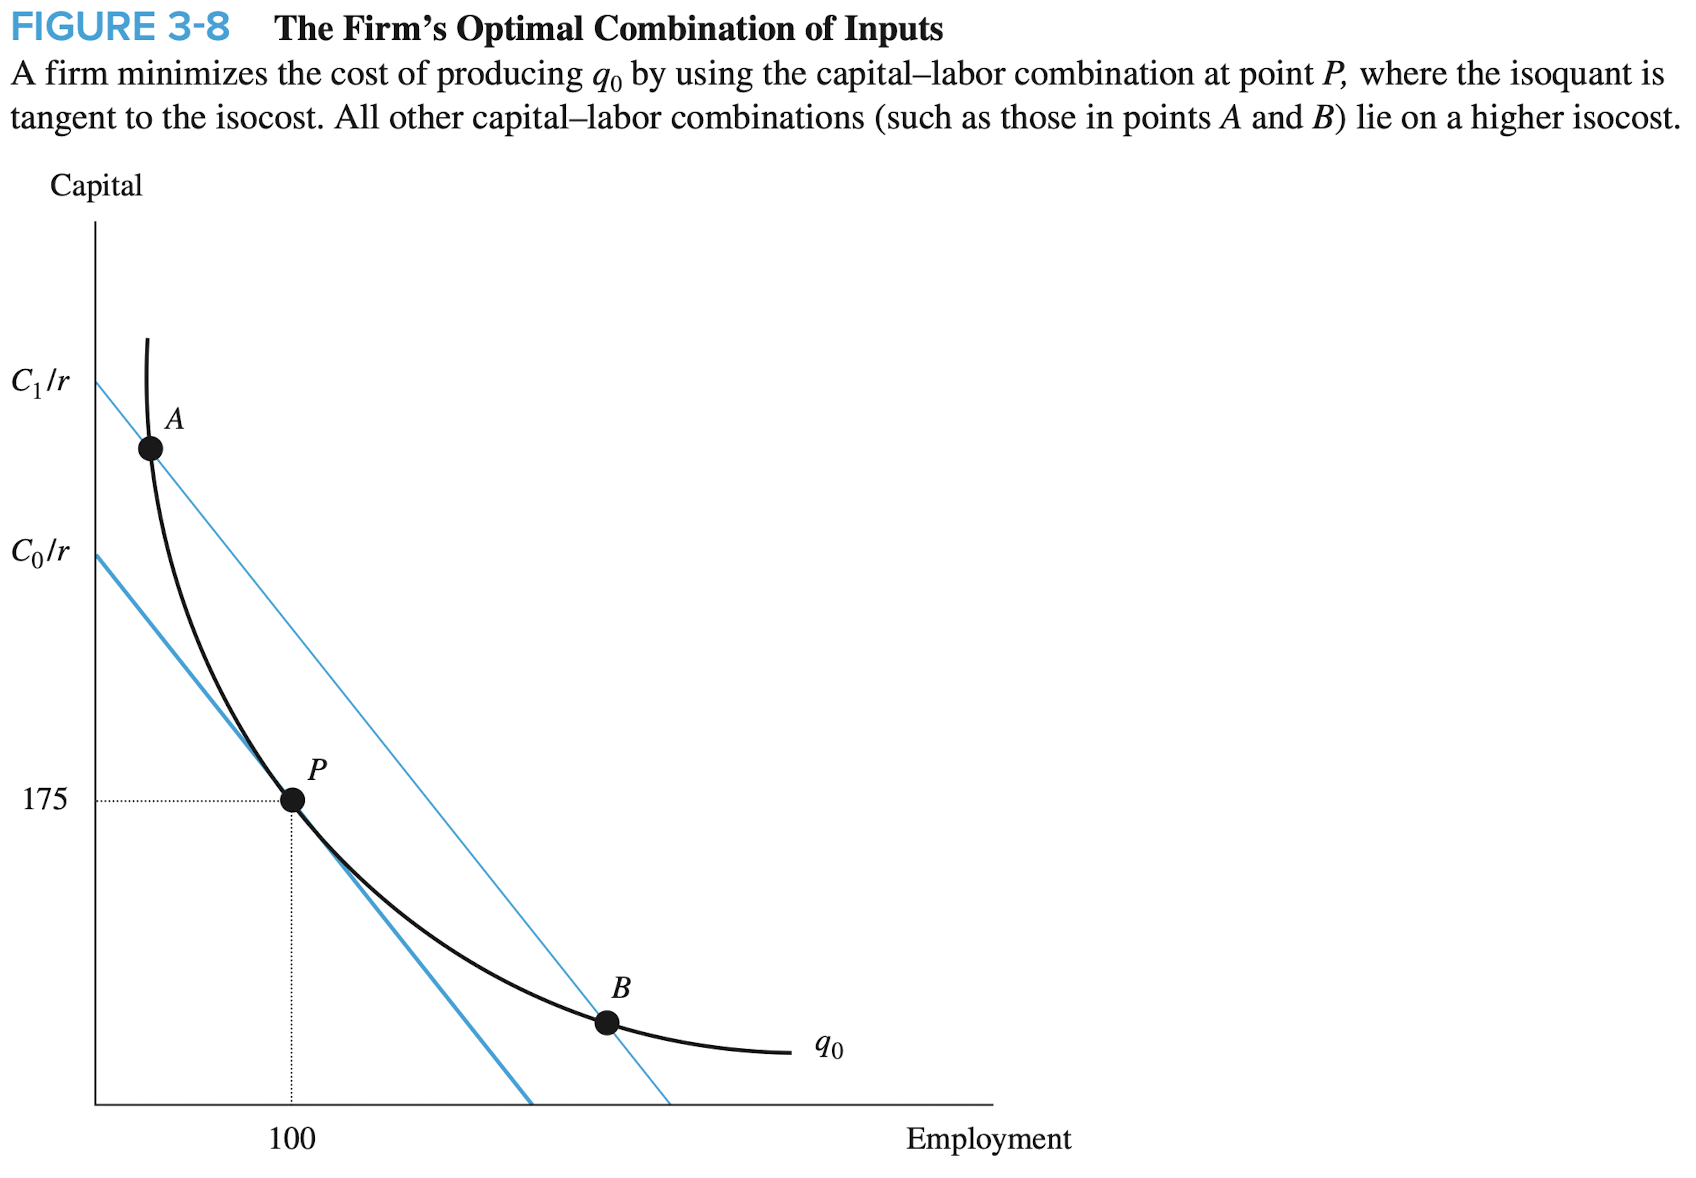
\includegraphics[width=0.95\textwidth]{../input/ch_3p3_cost_min.png}
    \caption{Cost Minimization}
    \label{fig:ch_3p3_cost_min}
\end{figure}

\FloatBarrier

At the cost-minimizing solution, given the isoquant's tangency and 
the slope of each curve,
we have:

\begin{align}
    \frac{M P_E}{M P_K}=\frac{w}{r}
\end{align}

That is the ratio of the marginal product of 
labor and capital equals the ratio of 
the cost of labor and capital.

The intuition may be more clearly seen by:

\begin{align}
    \frac{M P_E}{w}=\frac{M P_K}{r} \label{eq:ch3_marg_prod_cost}
\end{align}

That is, the cost of the marginal product 
coming from labor and capital are equalized.
It's logical that this is the optimal point, since if 
the cost of the marginal product from one was 
lower than the other, then the firm should re-allocate
its spending toward that input.

\paragraph{Long-Run Profit Maximization}

Note that the condition given by \eqref{eq:ch3_marg_prod_cost} 
is not the same as 
saying that firms maximize profit.
This condition is only saying how firms 
minimize cost given a particular selection of output.
Maximizing profit also requires choosing the optimal
level of output.

Long-run profit maximization also necessitates that

\begin{align}
    w=p \times M P_E \quad \text { and } \quad r=p \times M P_K
\end{align}

which implies \eqref{eq:ch3_marg_prod_cost}, but the 
reverse is not true.

\begin{questions}
    Do we have a way of indicating the process 
    of finding the profit-maximizing point on
    the isoquant-isocost diagram?
\end{questions}

%%%%%%%%%%%%%%%%%%%%%%%%%%%%%%%%%%%%%%%%%%%%%%%%%%%%%%%%%%%%%%%%%%%%%%%%%%%%%%%%%%%%%%%
%%%%%%%%%%%%%%%%%%%%%%%%%%%%%%%%%%%%%%%%%%%%%%%%%%%%%%%%%%%%%%%%%%%%%%%%%%%%%%%%%%%%%%%
\subsection{The Long-Run Demand Curve for Labor}

Suppose that the wage for workers 
falls.
How will firms respond in the long run?
First, note that the worker's wage falling 
corresponds to a flattening of the 
isocost line (where the number of workers 
is on the $x$-axis).

Our first reaction to try to 
understand how the firms will re-allocate between capital 
and workers may be to draw 
\autoref{fig:ch_3p4_naive_adj}. However, 
this would be the wrong 
approach. In particular, this presupposes 
that the firm is going to hold costs fixed, but 
there is no reason to believe that this is the case.

\FloatBarrier

\begin{figure}[!htb]
    \centering
        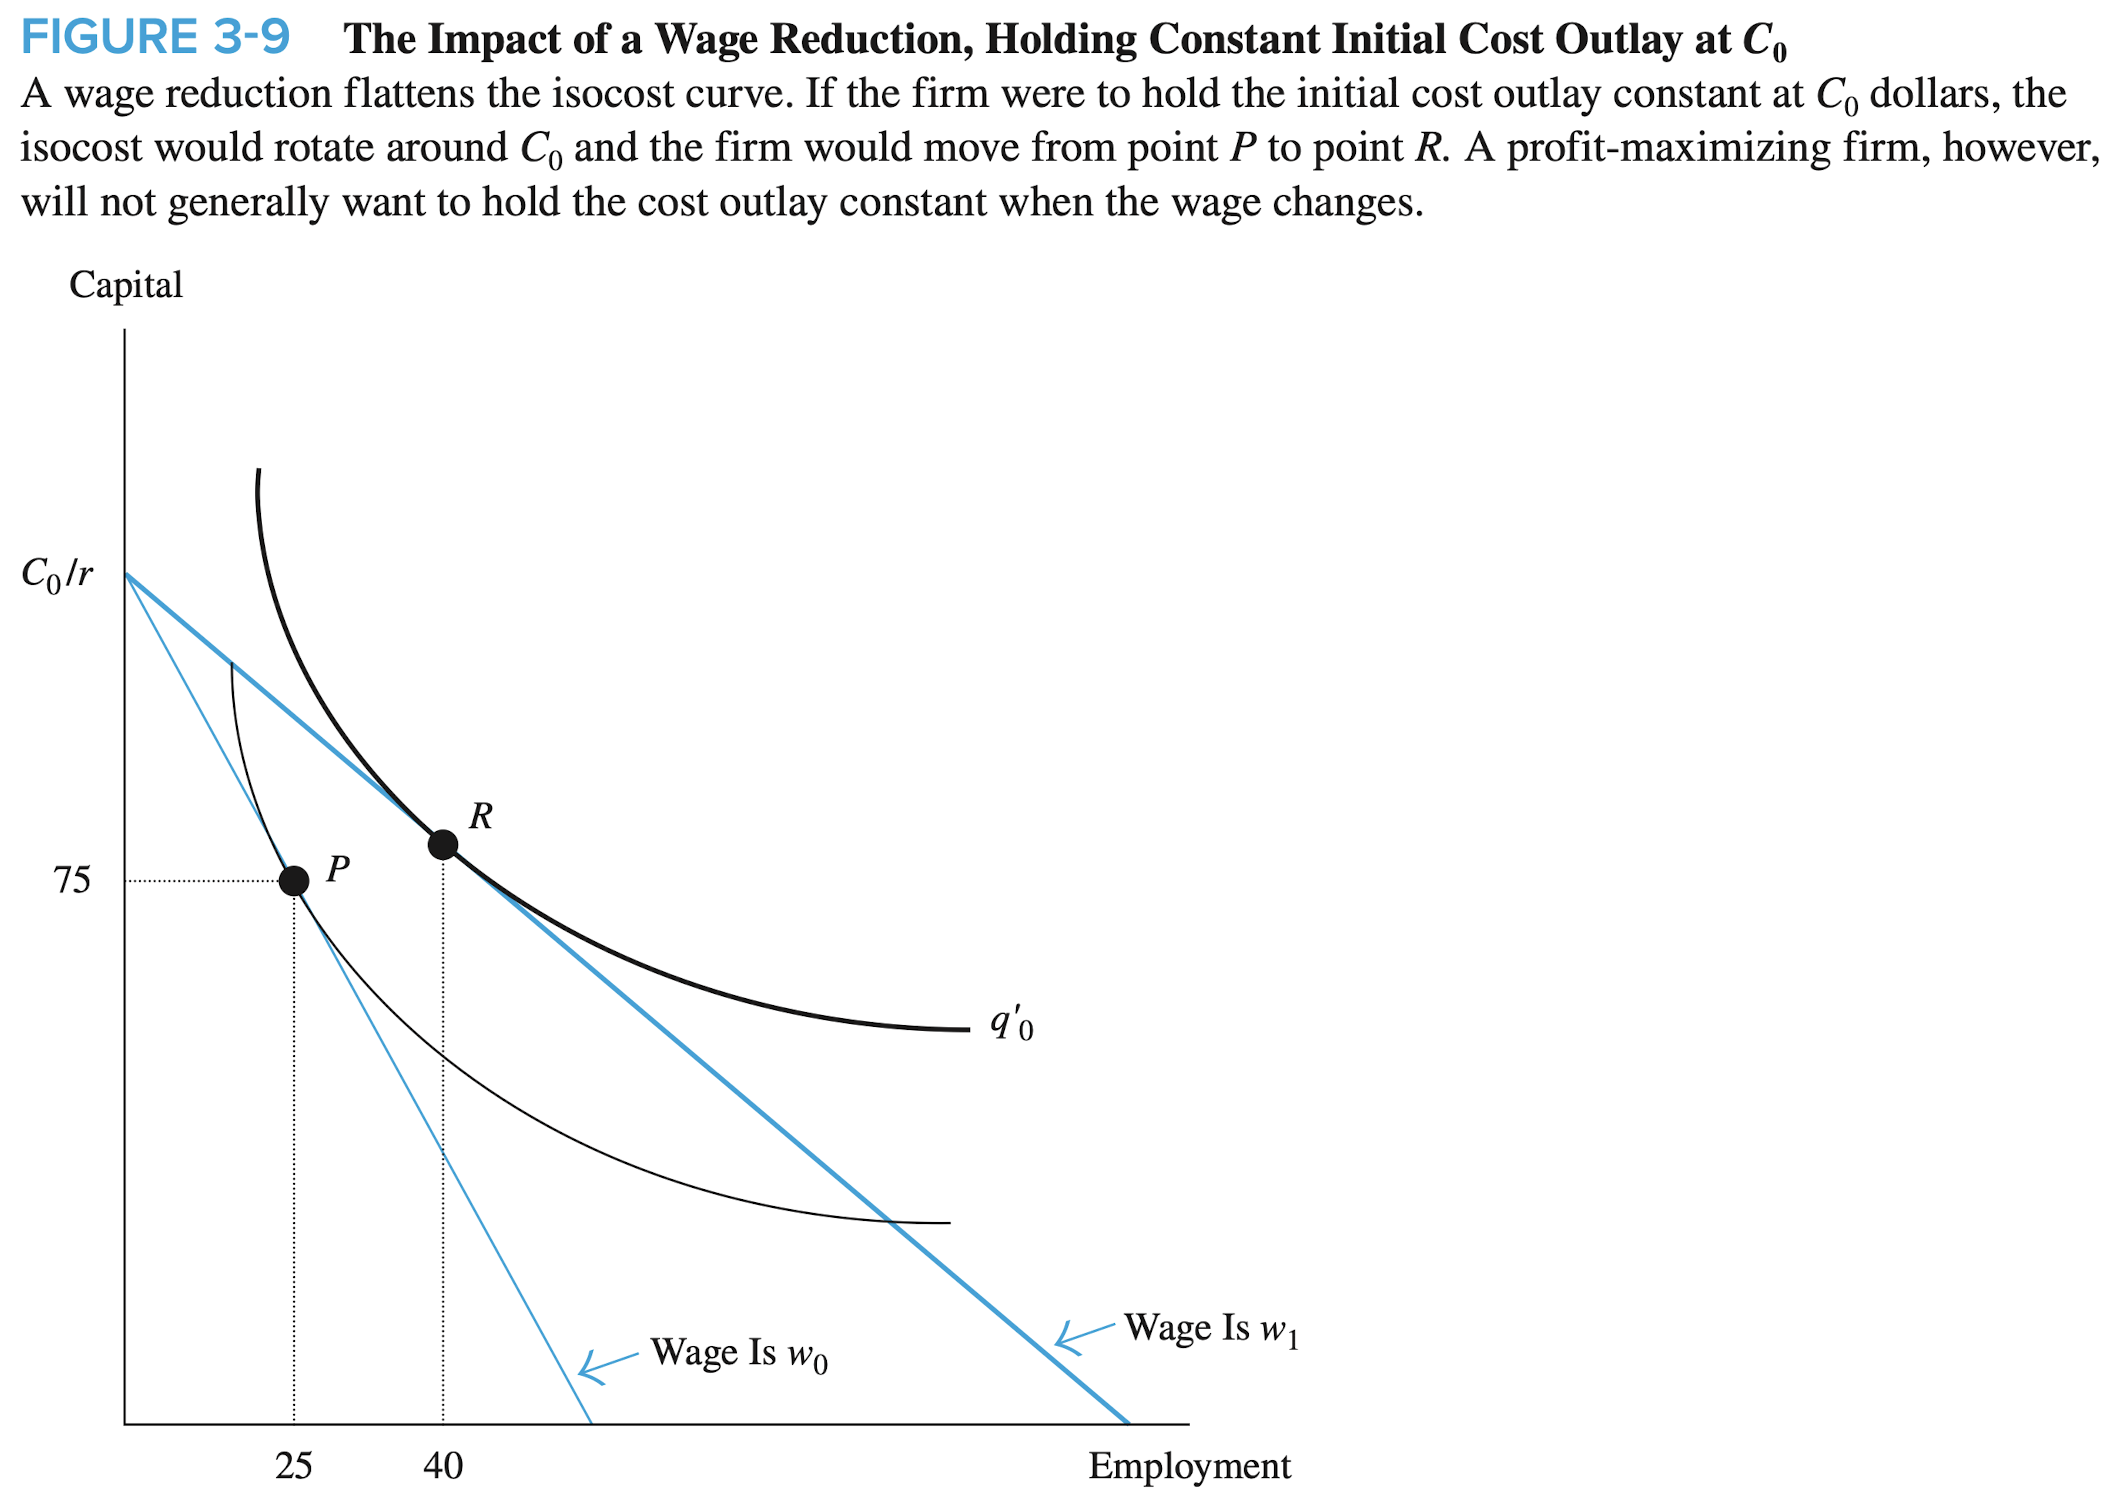
\includegraphics[width=0.95\textwidth]{../input/ch_3p4_naive_adj.png}
    \caption{The Impact of a Wage Decrease if $C_0$ is Fixed}
    \label{fig:ch_3p4_naive_adj}
\end{figure}

\FloatBarrier

%%%%%%%%%%%%%%%%%%%%%%%%%%%%%%%%%%%%%%%%%%%%%%%%%%%%%%%%%%%%%%%%%%%%%%%%%%%%%%%%%%%%%%%
\subsubsection{Will the Firm Expand if the Wage Falls?}

Accommodating the reality that 
the cost may change, we can look
to \autoref{fig:ch_3p4_alt_adj} for an example 
of what might happen.
Specifically, the fact that the marginal cost 
curve has shifted down encourages the 
firm to increase production. (See Panel (a).)
Then, we can look at the relevant isoquant and isocost 
in Panel (b) to see what's happened to employment 
and capital usage. In this example, we display 
both as having increased. The important takeaway here, 
though, is primarily just that the firm is 
producing at a different level of cost.

\FloatBarrier

\begin{figure}[!htb]
    \centering
        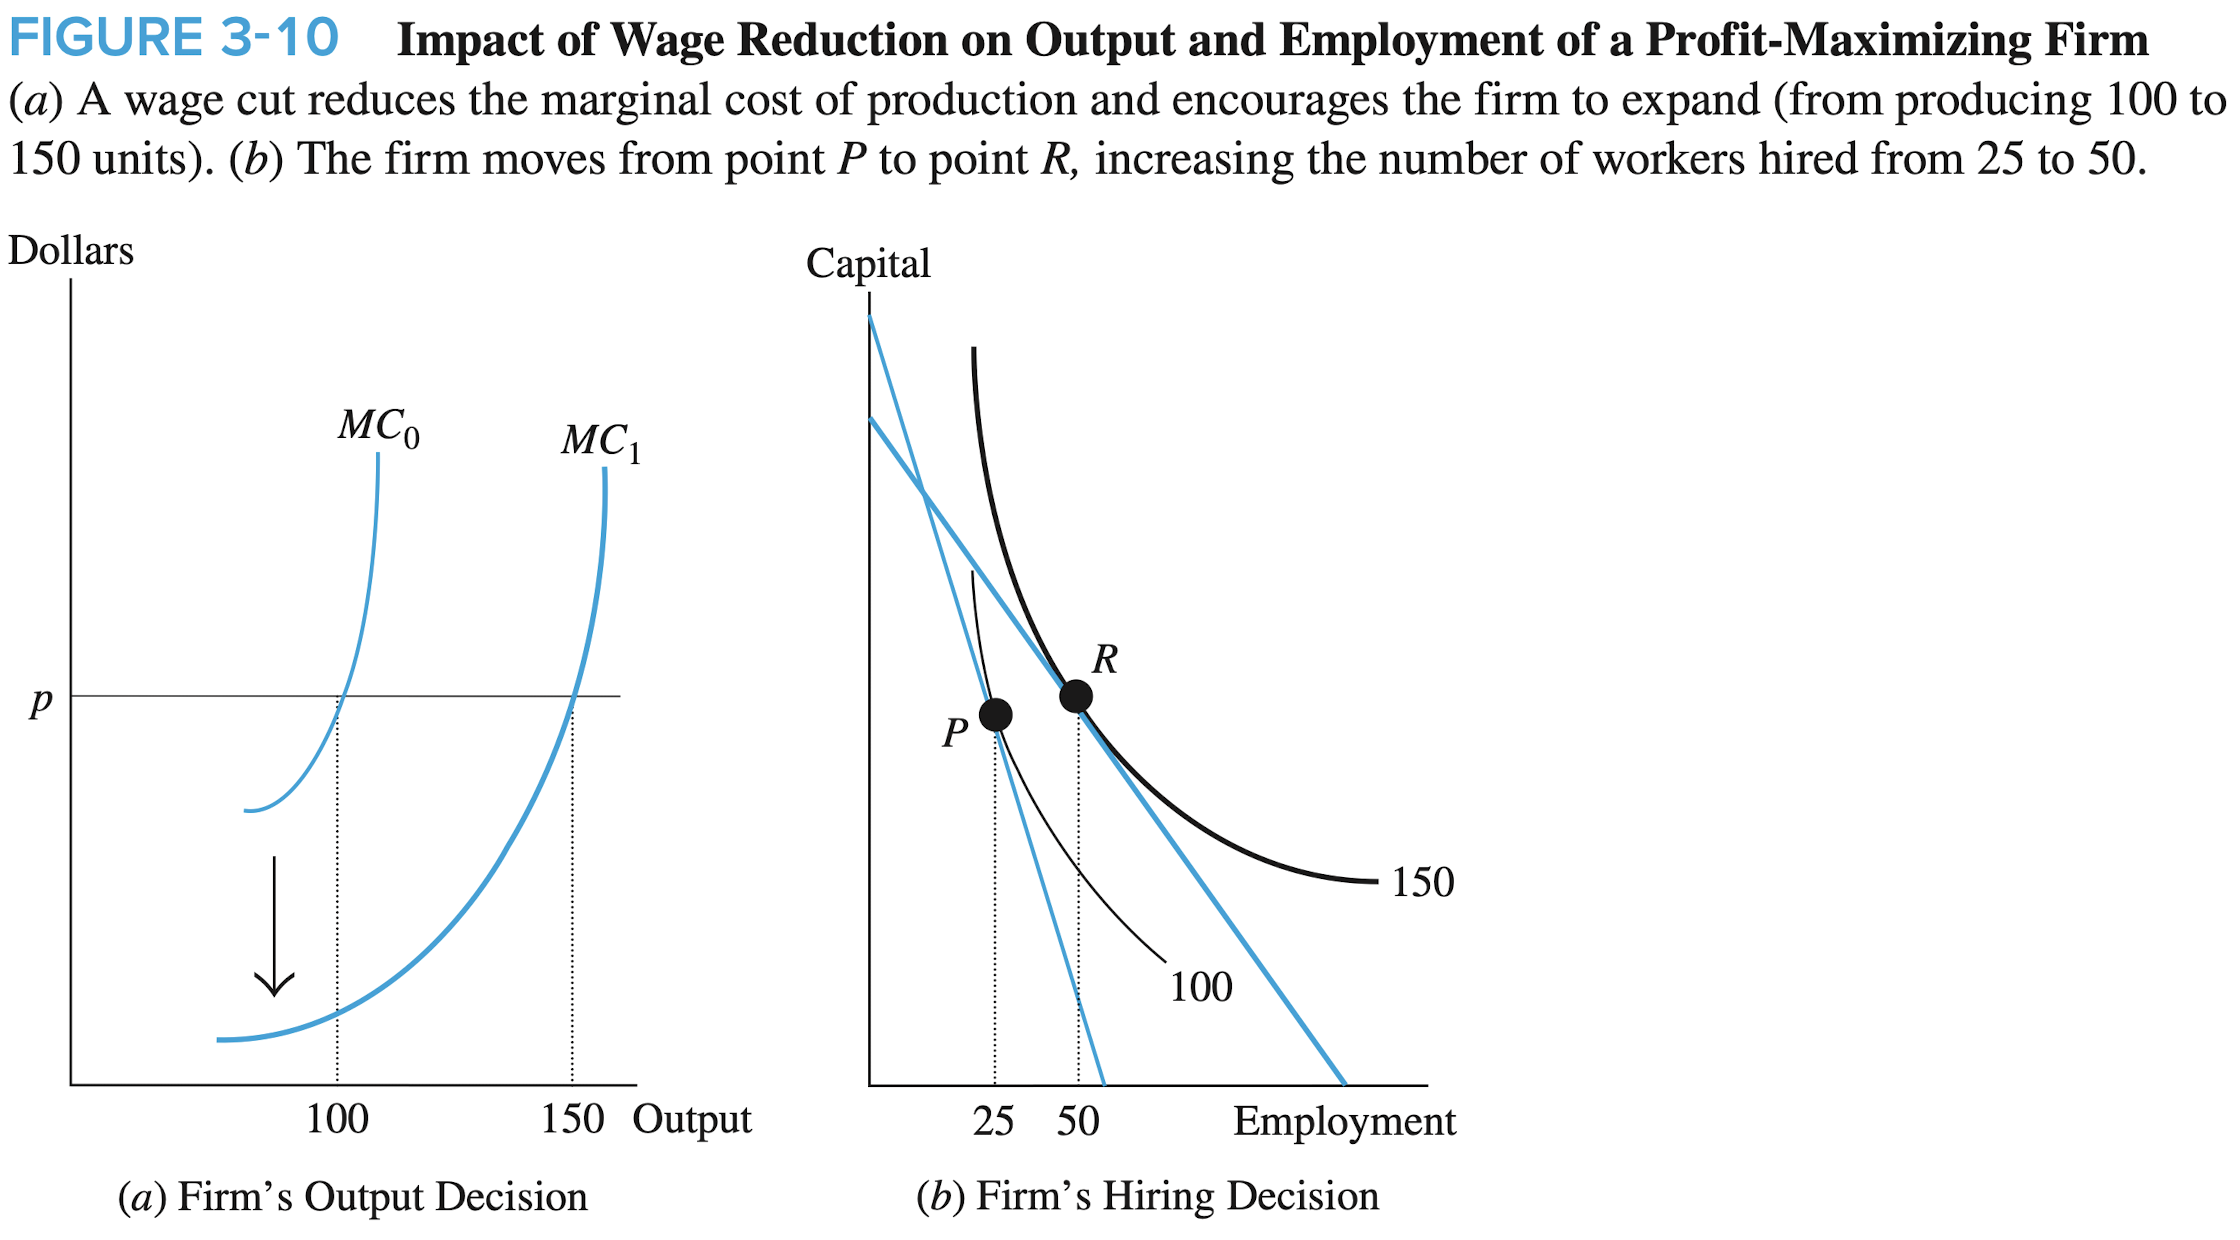
\includegraphics[width=0.95\textwidth]{../input/ch_3p4_alt_adj.png}
    \caption{The Impact of a Wage Decrease if $C_0$ is Not Fixed}
    \label{fig:ch_3p4_alt_adj}
\end{figure}

\FloatBarrier

%%%%%%%%%%%%%%%%%%%%%%%%%%%%%%%%%%%%%%%%%%%%%%%%%%%%%%%%%%%%%%%%%%%%%%%%%%%%%%%%%%%%%%%
\subsubsection{Substitution and Scale Effects}

This section is analogous to our discussion 
of income and substitution effects for 
consumers. Here, we consider two effects that 
accompany a change in an input price for a 
firm: the scale effect and the substitution effect.

\begin{definition}[Scale Effect] 
    
    The scale effect refers to what 
    happens to the firm's demands for its inputs
    as production increases, holding input prices constant.

\end{definition}

\begin{definition}[Substitution Effect] 
    
    The substitution effect refers to what 
    happens to the firm's demands for its inputs
    as input prices change, holding production constant.
    
\end{definition}

In \autoref{fig:ch_3p4_sub_scale_effects},
we illustrate these two effects
in the context of a wage decrease.
Prior to the wage change, the firm chooses 
employment and capital levels corresponding to 
$P$. If the production were shifted to the new 
level (150, in this example), holding input prices constant,
the firm would choose the point $Q$, which
corresponds to an increase in both capital 
and employment. This is the scale effect. The increase 
in both inputs holds as long as both are ``normal inputs.''
However, if we now adjust the input prices
to reflect the wage decrease, holding production constant
at this new level, the firm would 
produce at point $R$. This 
reflects a decline in capital usage, relative to $Q$,
and an increase in employment. 
This is the substitution effect. The directional effect of the 
substitution effect is not ambiguous.



Scale Effect note: When one input (labor) becomes cheaper, the firm's unit cost falls. 
This lowers the output price needed to break even, so the 
firm profitably expands production. Producing more output 
requires more of all inputs in the cost-minimizing mix at the 
new prices. That outward shift in input demand due purely to 
producing more is the scale effect. Complementarity—where 
extra labor raises the marginal product of capital—can further 
boost capital demand, but it's not necessary for the scale effect to operate.

Take for example, a Leontief production function, 
where inputs are used in fixed proportions.
In this case, there is no substitution effect.
However, because the unit price decreases, 
the firm will still expand production,
requiring more of both inputs, capturing 
purely a scale effect.

Note of effects together: ``When the price of one 
input falls, the cost to produce an extra unit falls, so the firm 
will produce more. The scale effect captures the fact that
the firm wants more of all inputs to produce more; this is 
strongest when inputs are complements.
However, the substitution effect captures that the firm will
want to use more of the input that has become cheaper and less
of the input that has become relatively more expensive.''



\FloatBarrier

\begin{figure}[!htb]
    \centering
        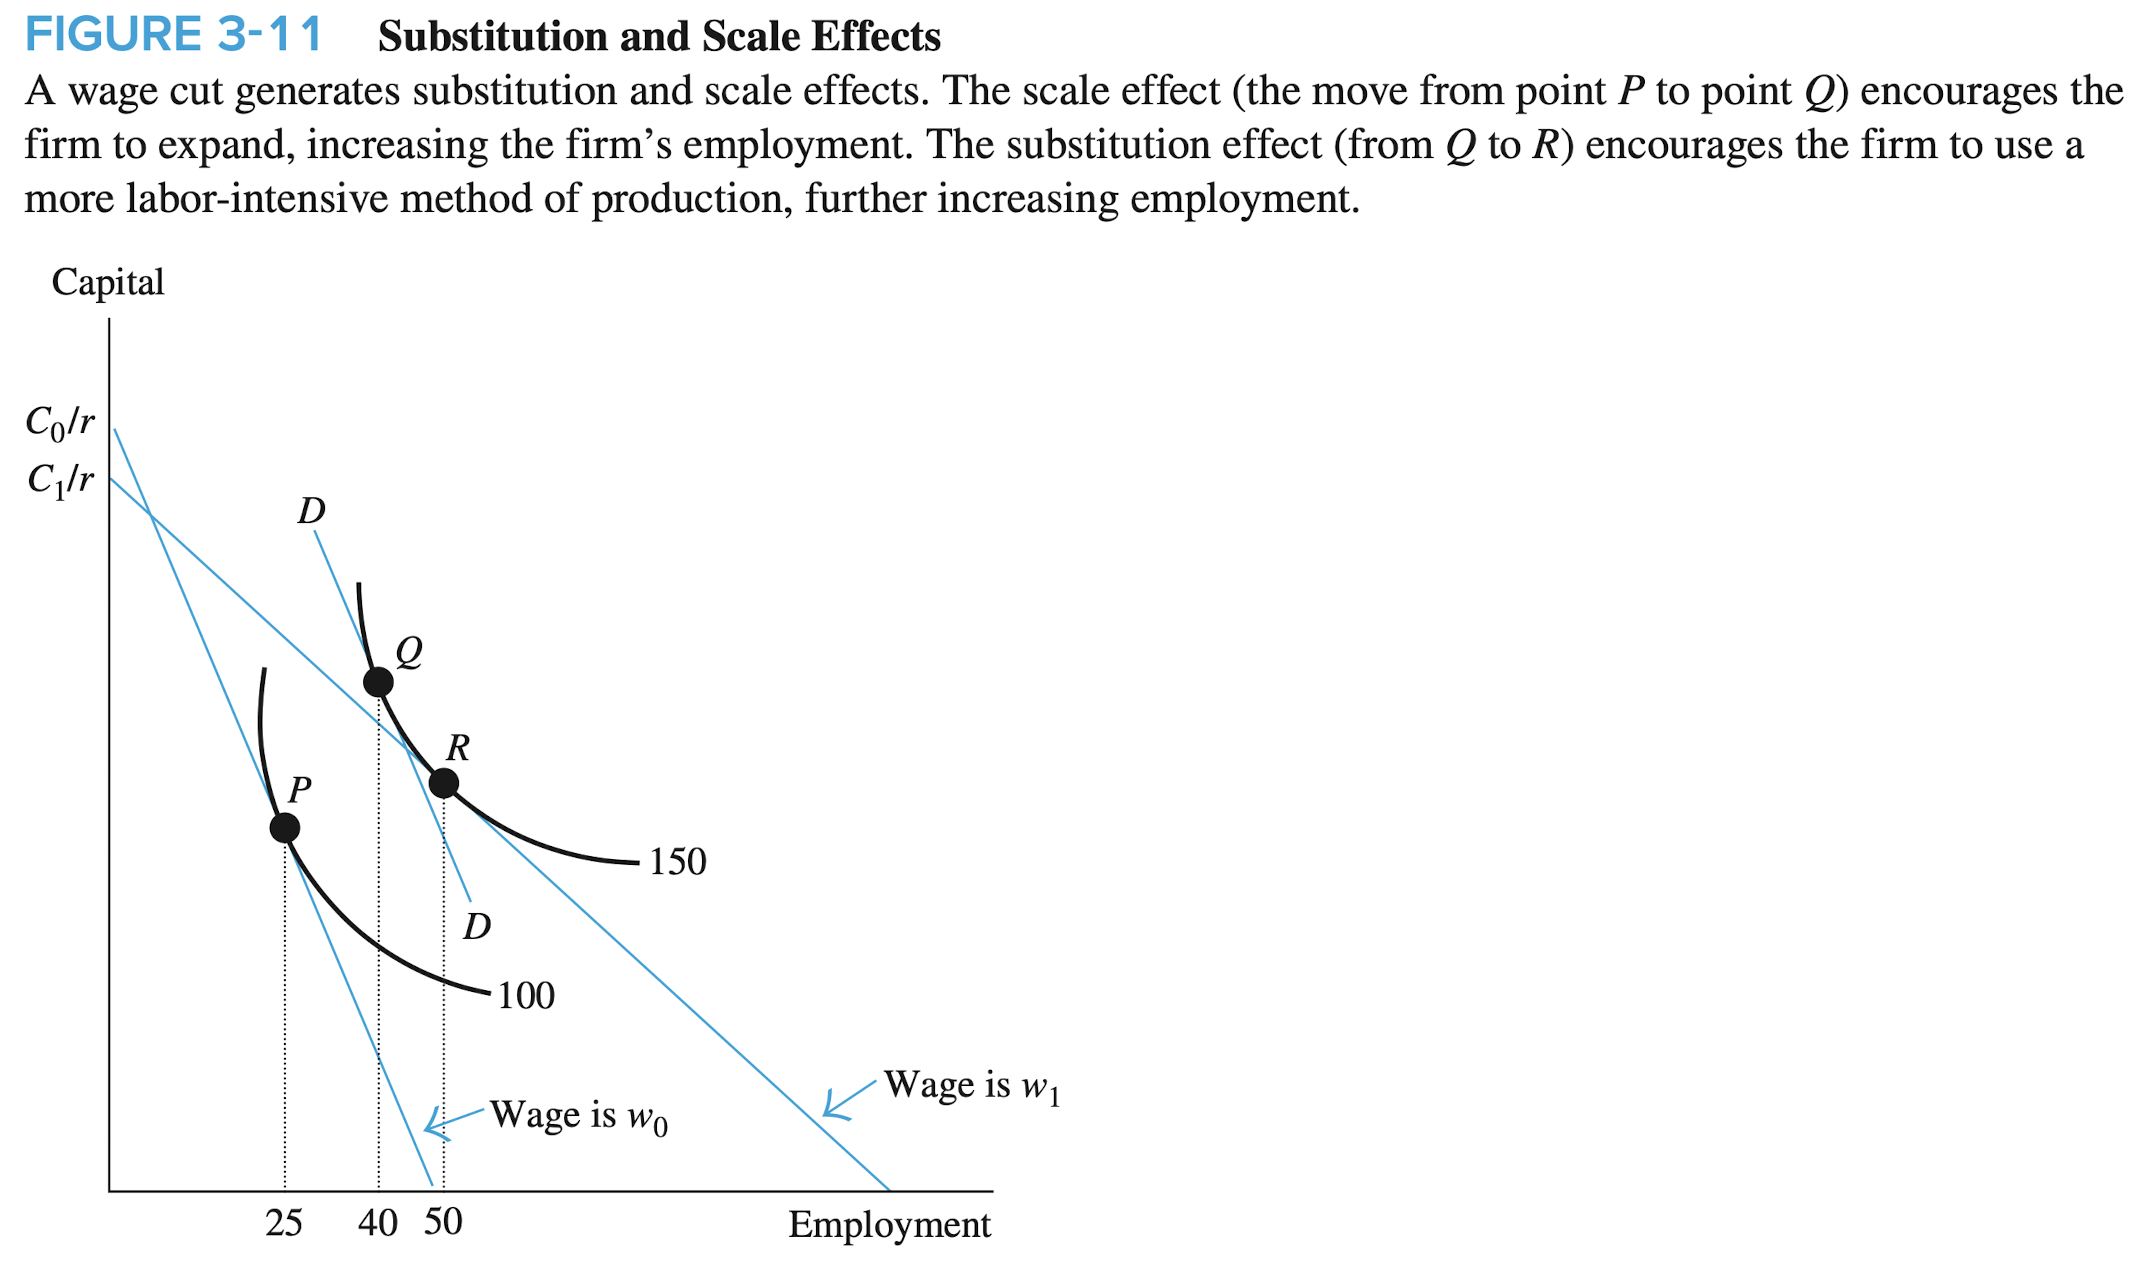
\includegraphics[width=0.95\textwidth]{../input/ch_3p4_sub_scale_effects.png}
    \caption{Substitution and Scale Effects}
    \label{fig:ch_3p4_sub_scale_effects}
\end{figure}

\FloatBarrier


\begin{definition}[Long-Run Elasticity of Labor Demand]

    The long-run elasticity of labor demand ($\delta_{LR}$)
    is the percentage change in the quantity of labor demanded in the
    long run ($E_{LR}$)
    resulting from a percentage change in the wage rate.
    
    \begin{align}
        \delta_{L R}=\frac{\Delta E_{L R} / E_{L R}}{\Delta w / w}=\frac{\Delta E_{L R}}{\Delta w} \cdot \frac{w}{E_{L R}}
    \end{align}
    
\end{definition}


In general, long-run labor demand will be more 
elastic than short-run labor demand. This dynamic is 
because in the long run, firms can adjust 
both capital and labor, so they can 
substitute between the two inputs.

\FloatBarrier

\begin{figure}[!htb]
    \centering
        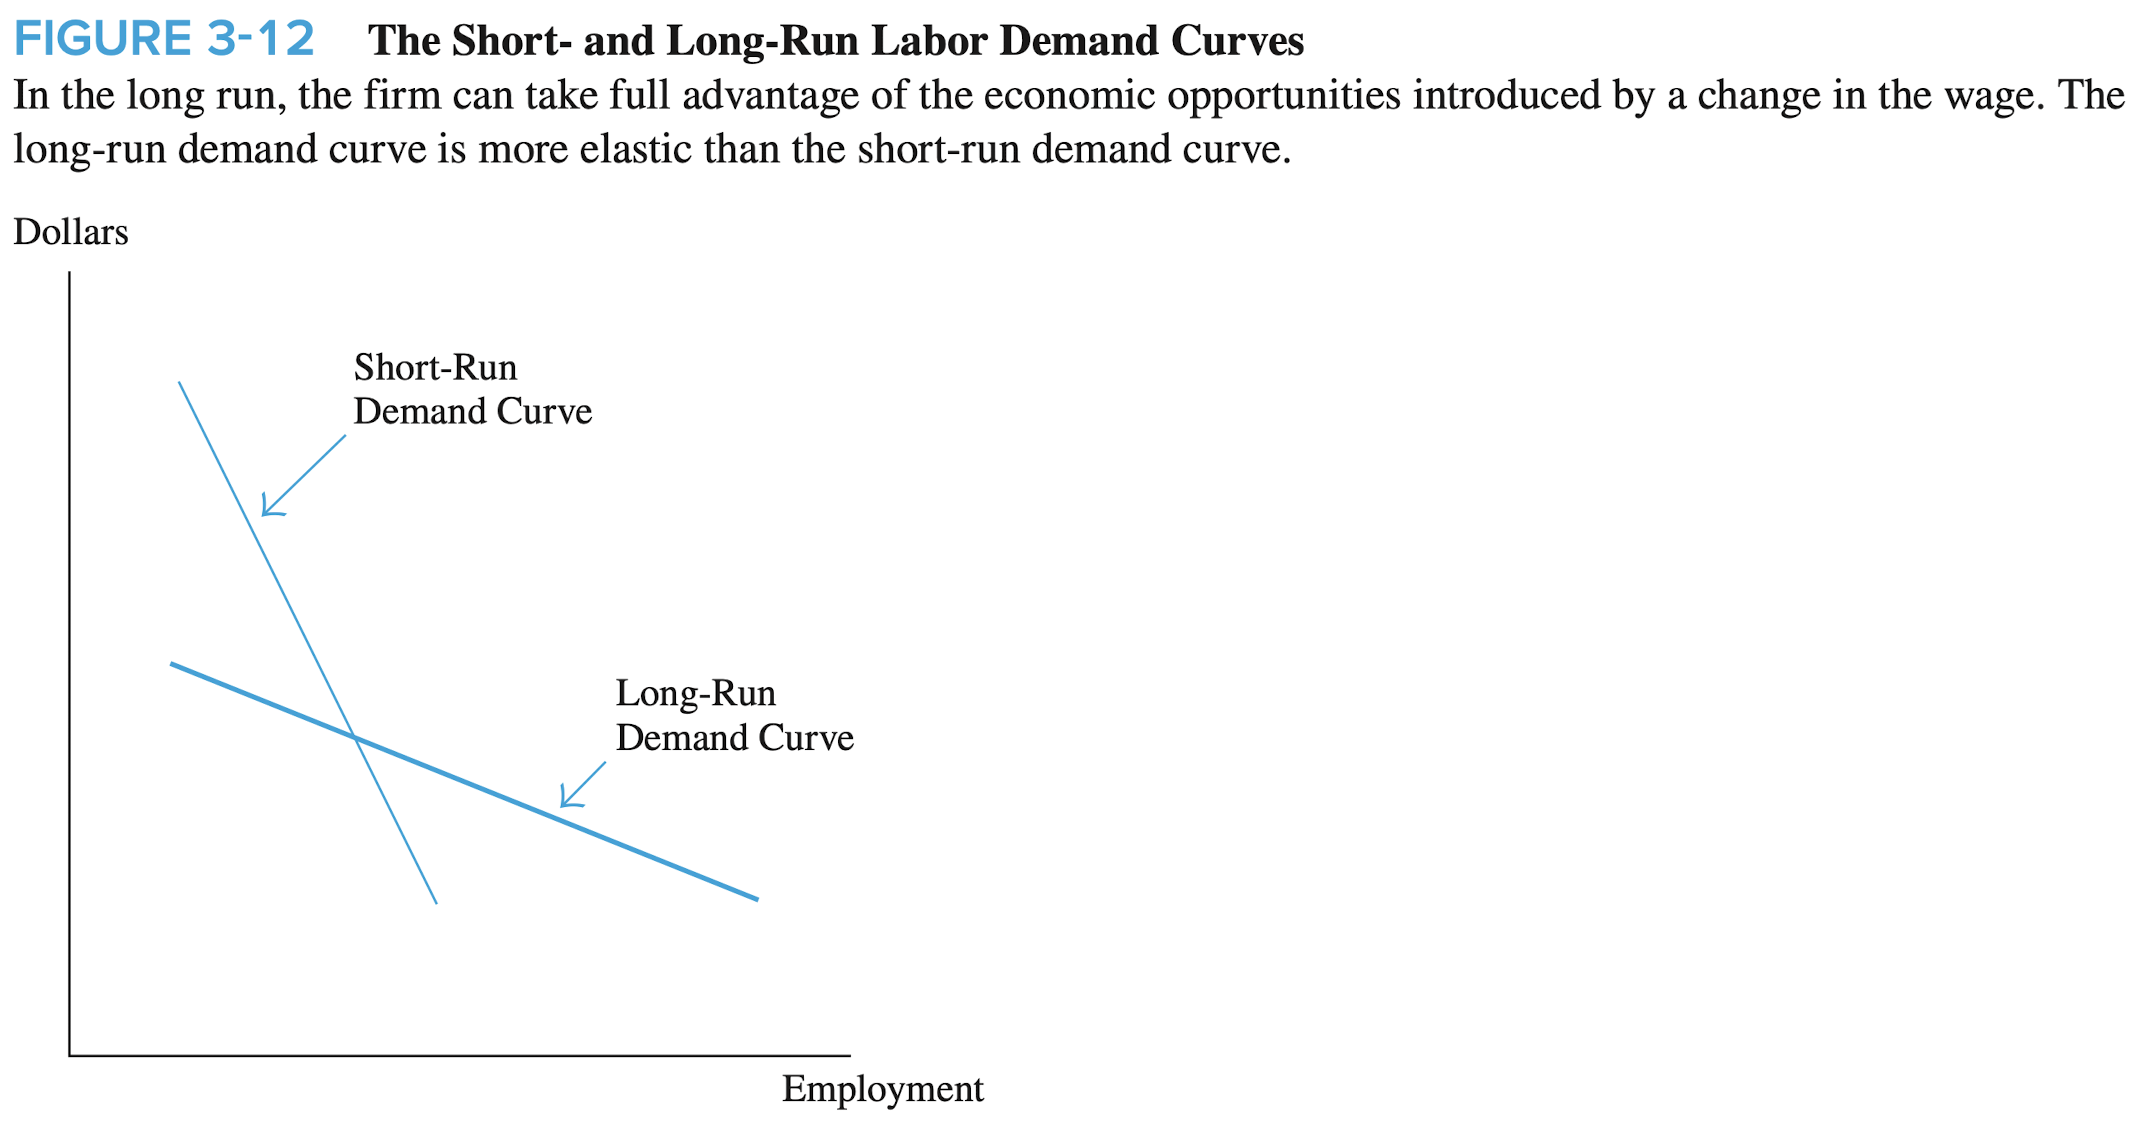
\includegraphics[width=0.95\textwidth]{../input/ch_3p4_long_v_short_run.png}
    \caption{Long-Run vs Short-Run Elasticity of Labor Demand}
    \label{fig:ch_3p4_long_v_short_run}
\end{figure}

\FloatBarrier

%%%%%%%%%%%%%%%%%%%%%%%%%%%%%%%%%%%%%%%%%%%%%%%%%%%%%%%%%%%%%%%%%%%%%%%%%%%%%%%%%%%%%%%
\subsubsection{Estimates of the Elasticity of Labor Demand}

The author suggests that the short-run 
elasticity of labor demand is in the range of 
-0.4 and -0.5. That is, a 10\% increase in wages
leads to a 4-5\% decrease in employment. 
He suggests that the long-run elasticity
is estimated to be around -1\%, i.e.,
a 10\% increase in wages leads to a 10\% decrease in employment.


%%%%%%%%%%%%%%%%%%%%%%%%%%%%%%%%%%%%%%%%%%%%%%%%%%%%%%%%%%%%%%%%%%%%%%%%%%%%%%%%%%%%%%%
%%%%%%%%%%%%%%%%%%%%%%%%%%%%%%%%%%%%%%%%%%%%%%%%%%%%%%%%%%%%%%%%%%%%%%%%%%%%%%%%%%%%%%%

\subsection{The Elasticity of Substitution}


``The size of the firm's substitution effect depends on the curvature of the isoquant.''

\begin{definition}[Perfect Substitute]
    
    If the isoquants are linear, 
    then the inputs are perfect substitutes.

\end{definition}

In the case of perfect substitutes, 
firms will simply use the cheapest input.

\begin{definition}[Perfect Complement]
    
    If the isoquants are right angles, 
    then the inputs are perfect complements.
    
\end{definition}

In the case of perfect complements,
firms will use inputs in fixed proportions.

See \autoref{fig:ch_3p4_perfect_sub_comp}
for an illustration of perfect substitutes
and perfect complements.

\FloatBarrier

\begin{figure}[!htb]
    \centering
        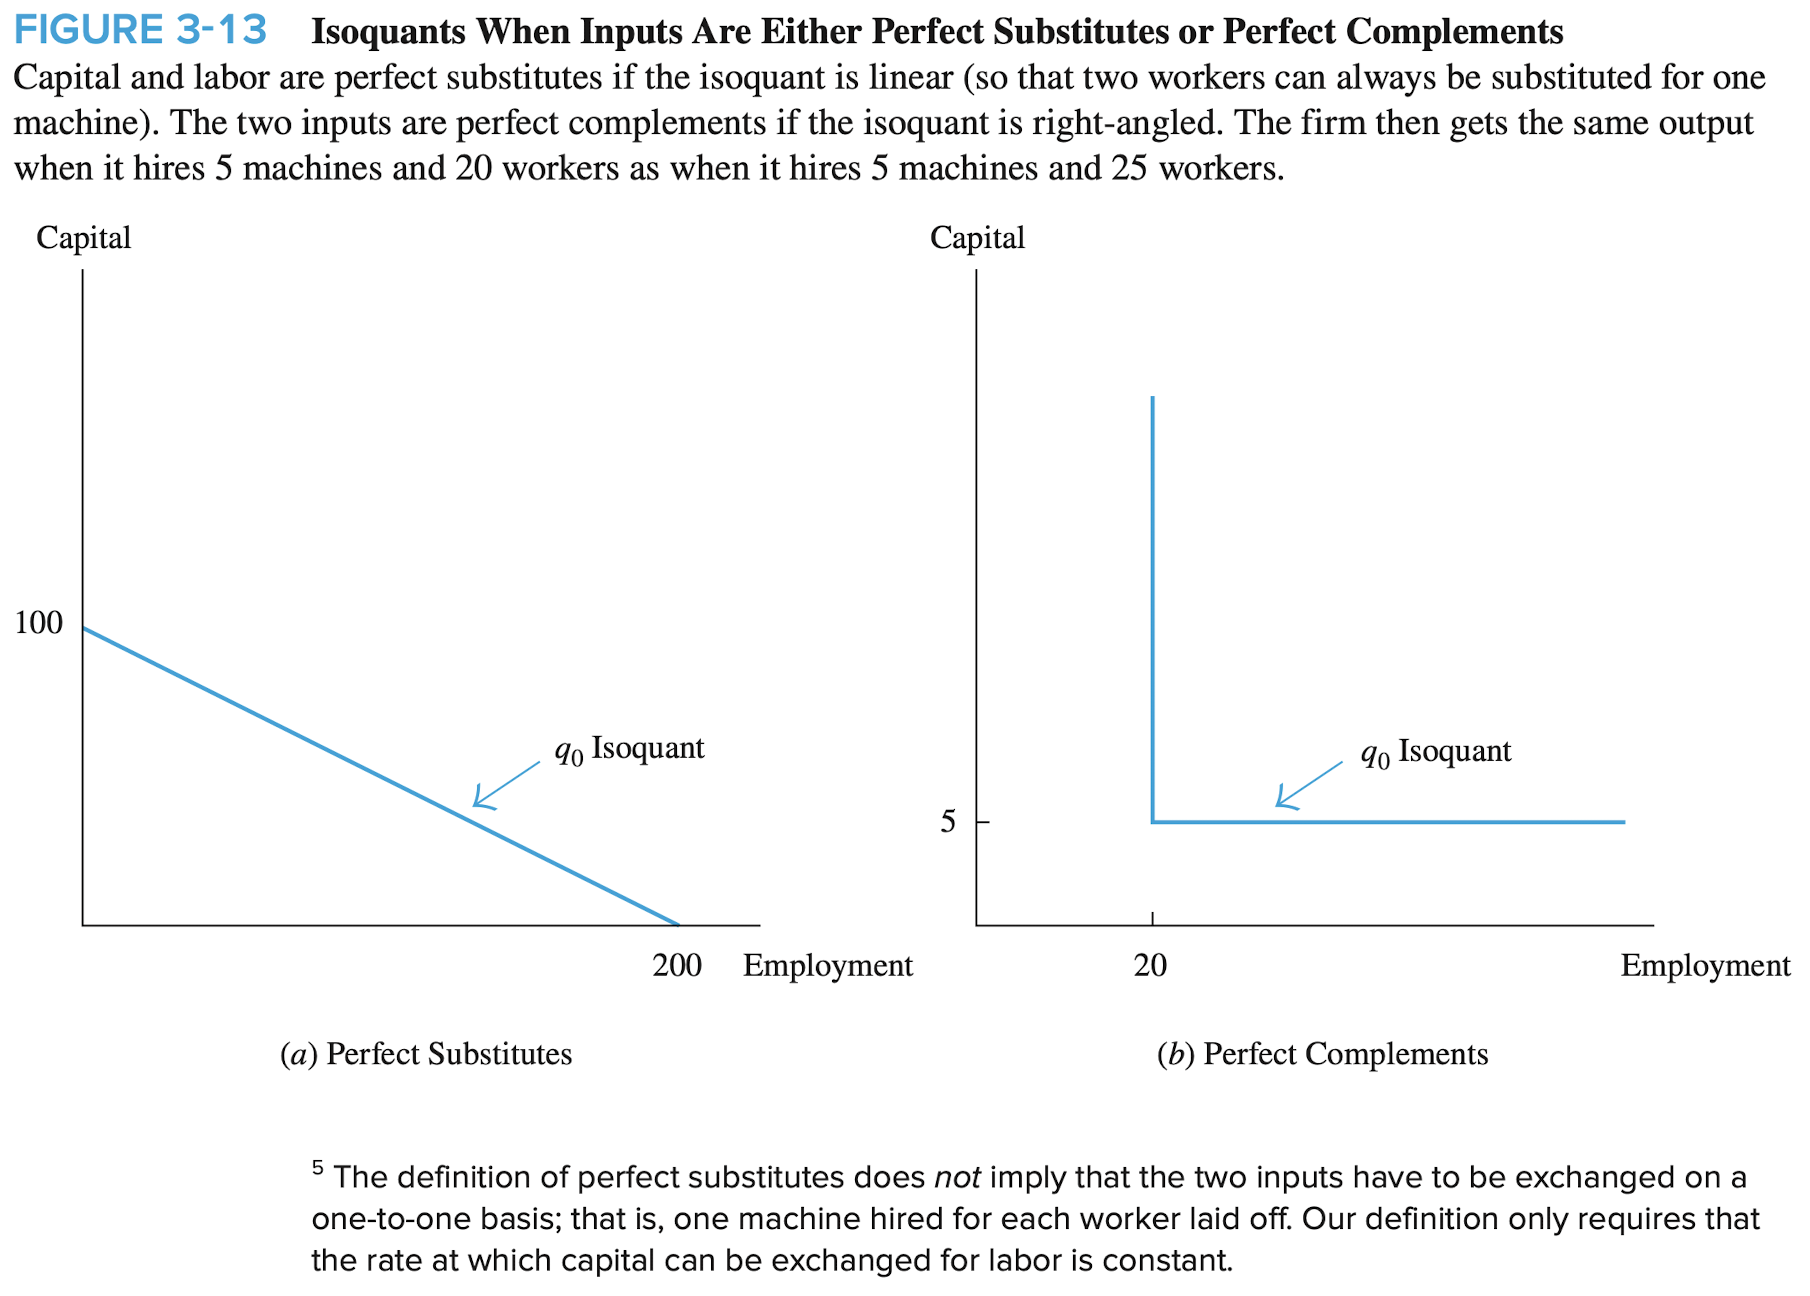
\includegraphics[width=0.95\textwidth]{../input/ch_3p4_perfect_sub_comp.png}
    \caption{Perfect Substitutes and Perfect Complements}
    \label{fig:ch_3p4_perfect_sub_comp}
\end{figure}

\FloatBarrier



\begin{definition}[Elasticity of Subsitution]

    The elasticity of substitution ($\sigma$)
    is the percentage change in the
    capital-labor ratio ($K/L$)
    resulting from a percentage change in the
    capital-labor price ratio ($w/r$).
    
    \begin{align}
        \sigma=\frac{\text { Percent change in } K / L}{\text { Percent change in } w / r}
    \end{align}
    
\end{definition}


%%%%%%%%%%%%%%%%%%%%%%%%%%%%%%%%%%%%%%%%%%%%%%%%%%%%%%%%%%%%%%%%%%%%%%%%%%%%%%%%%%%%%%%
%%%%%%%%%%%%%%%%%%%%%%%%%%%%%%%%%%%%%%%%%%%%%%%%%%%%%%%%%%%%%%%%%%%%%%%%%%%%%%%%%%%%%%%
\subsection{What Makes Labor Demand Elastic?}


Marshall's rules of derived demand 
describe situations in which we would 
expect labor demand to be more elastic: 

\begin{enumerate}
    \item ``Labor demand is more elastic the greater the elasticity of substitution.''
    \item ``Labor demand is more elastic the greater the elasticity of demand for the output.''
    \item ``Labor demand is more elastic the greater labor's share in total costs.''
    \item ``The demand for labor is more elastic the greater the supply elasticity of other factors of production.''
\end{enumerate}


%%%%%%%%%%%%%%%%%%%%%%%%%%%%%%%%%%%%%%%%%%%%%%%%%%%%%%%%%%%%%%%%%%%%%%%%%%%%%%%%%%%%%%%
%%%%%%%%%%%%%%%%%%%%%%%%%%%%%%%%%%%%%%%%%%%%%%%%%%%%%%%%%%%%%%%%%%%%%%%%%%%%%%%%%%%%%%%
\subsection{Factor Demand with Many Inputs}

We now consider
extending the theory we've developed so far 
to more inputs than simply labor and capital.

Suppose the firm's production function 
is instead given by:

\begin{align}
    q=f\left(x_1, x_2, x_3, \ldots, x_n\right)
\end{align}

where each $x_i$ is a different input.
We denote the marginal product of input $i$ as $MP_i$,
and the price of input $i$ as $w_i$.

Under this setup, we still have the result that
the $i$th input is purchased up to the point that:

\begin{align}
    w_i=p \times MP_i
\end{align}

\begin{definition}[Cross-Elasticity of Factor Demand] 
    
    As a measure of how the demand for one input 
    responds to a change in the price of another input, 
    we consider the cross-elasticity of factor demand:

    \begin{align}
        \delta_{ij} = \frac{ \% \Delta x_i}{\% \Delta w_j}
    \end{align}

\end{definition}

If the cross-elasticity is positive, then we say that 
the two inputs are substitutes.
If the cross-elasticity is negative, then we say that
the two inputs are complements.

\begin{definition}[Capital-Skill Complementarity Hypothesis]
    
    The capital-skill complementarity hypothesis
    is the hypothesis that unskilled labor 
    and capital are substitutes, while
    skilled labor and capital are complements.
    
\end{definition}

%%%%%%%%%%%%%%%%%%%%%%%%%%%%%%%%%%%%%%%%%%%%%%%%%%%%%%%%%%%%%%%%%%%%%%%%%%%%%%%%%%%%%%%
%%%%%%%%%%%%%%%%%%%%%%%%%%%%%%%%%%%%%%%%%%%%%%%%%%%%%%%%%%%%%%%%%%%%%%%%%%%%%%%%%%%%%%%
\subsection{Overview of Labor Market Equilibrium}

We will cover it more fully in the next 
chapter, but now we will provide a brief overview of 
the idea of labor market equilibrium.
The main idea is that the labor market
occurs at the intersection of 
the labor supply and labor demand curves.

\autoref{fig:ch_3p8_eq}
shows an example of labor market equilibrium
at $(E^*, w^*)$. At this point, in contrast to 
any other wage, the number of workers 
who want to work equals the number of workers
that firms want to hire.

\FloatBarrier

\begin{figure}[!htb]
    \centering
        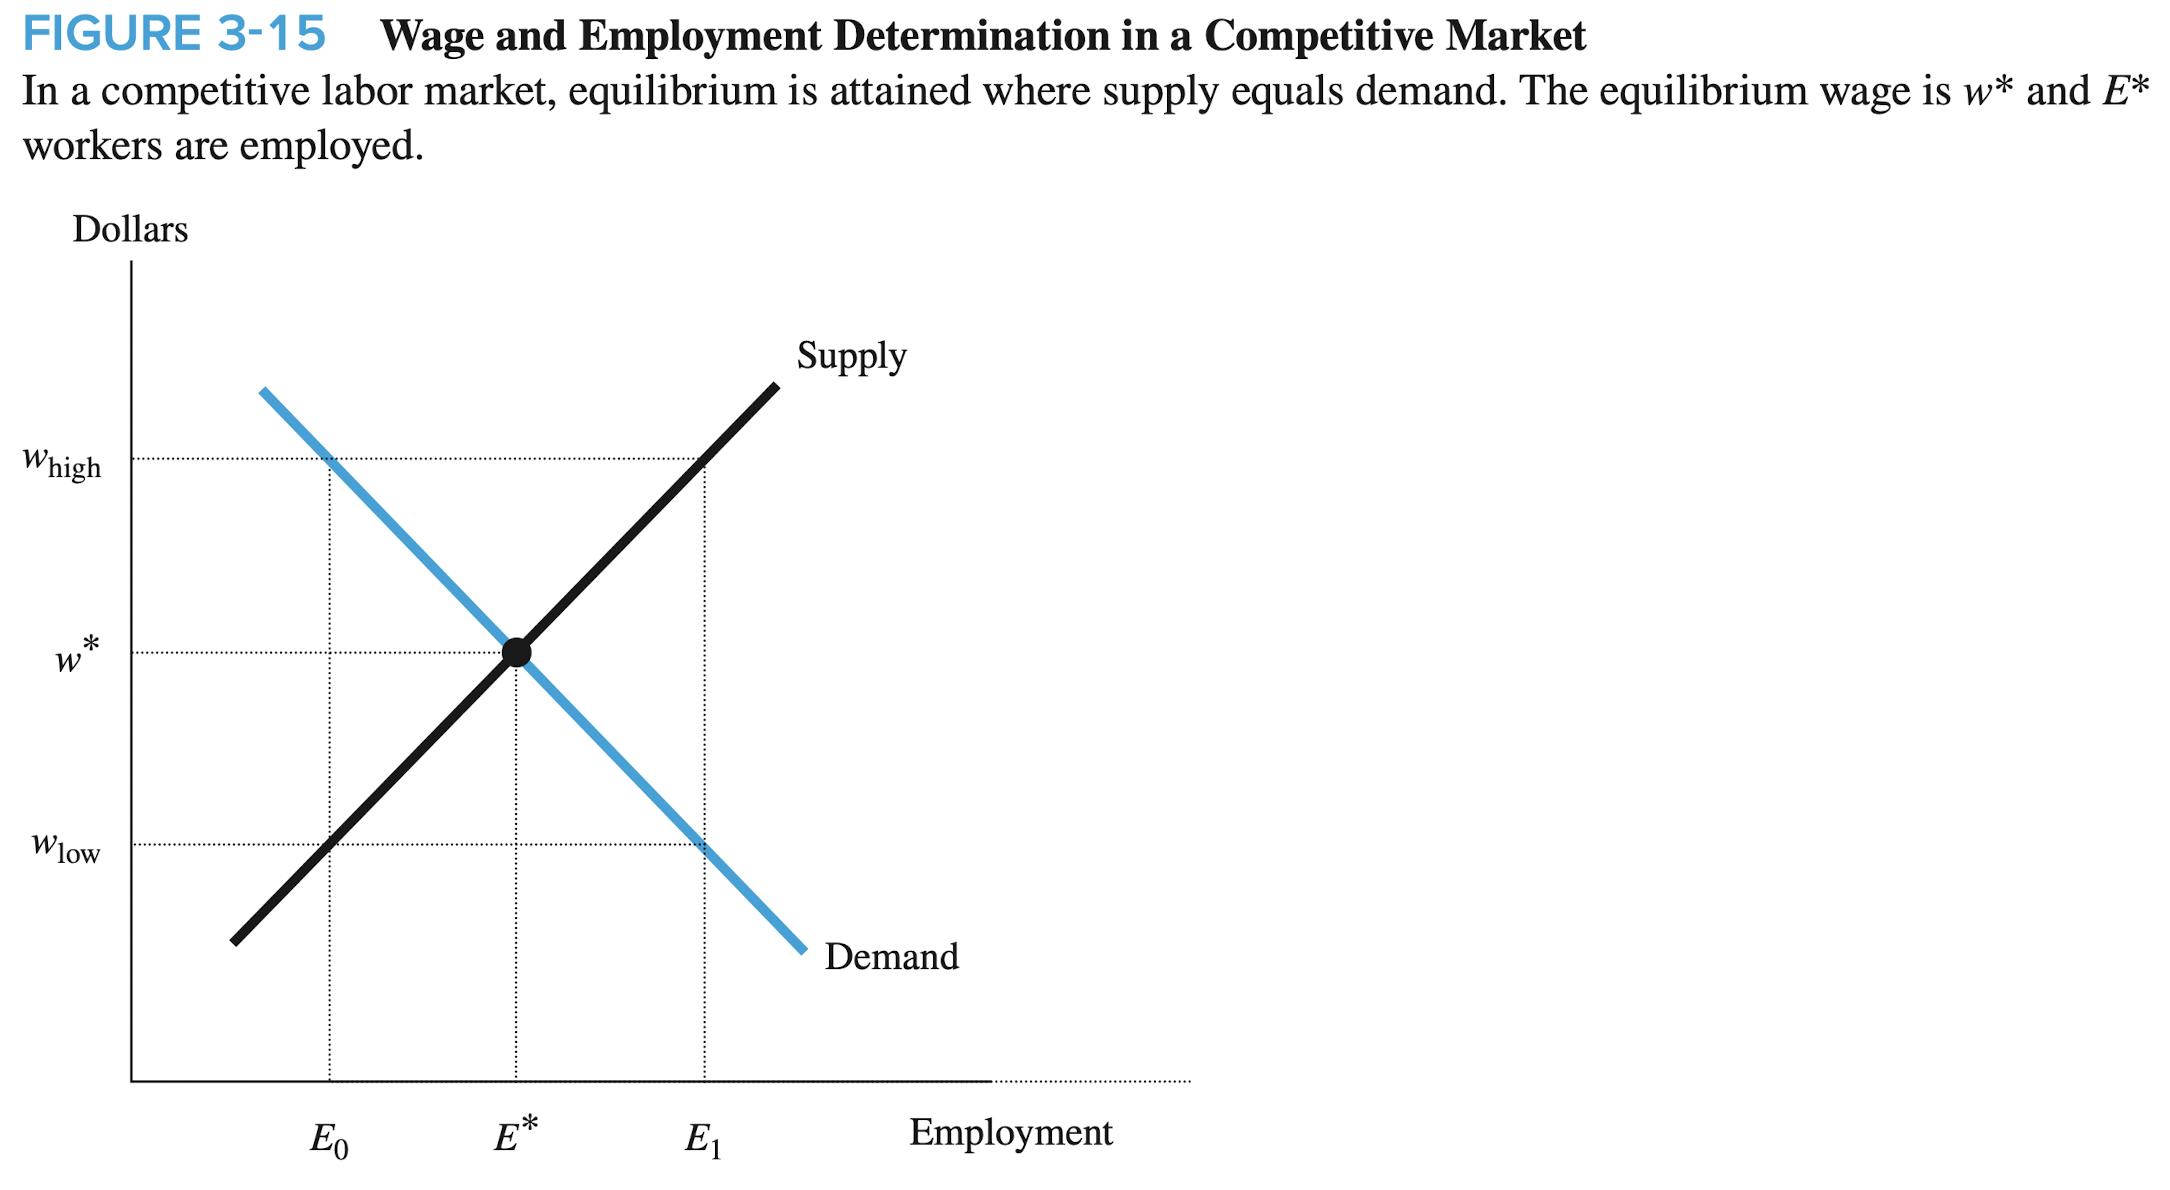
\includegraphics[width=0.95\textwidth]{../input/ch_3p8_eq.png}
    \caption{Labor Market Equilibrium Example}
    \label{fig:ch_3p8_eq}
\end{figure}

\FloatBarrier

%%%%%%%%%%%%%%%%%%%%%%%%%%%%%%%%%%%%%%%%%%%%%%%%%%%%%%%%%%%%%%%%%%%%%%%%%%%%%%%%%%%%%%%
%%%%%%%%%%%%%%%%%%%%%%%%%%%%%%%%%%%%%%%%%%%%%%%%%%%%%%%%%%%%%%%%%%%%%%%%%%%%%%%%%%%%%%%

\subsection{Rosie the Riveter as an Instrumental Variable}

The author notes that much of modern 
labor economics research is focused on 
estimating labor supply and demand curves for 
various groups.

One method for doing so is to identify an 
instrumental variable (IV) that shifts
only either supply or demand.
This shift can then be used to trace out 
the other. The logic of this 
approach is visualized in 
\autoref{fig:ch_3p9_instrument_dem}.
Suppose the supply and demand 
curves start at $S_0$ and $D_0$, respectively.
Then, consider three scenarios:

\begin{itemize}
    \item $S_0$ moves to $S_1$, while $D_0$ stays fixed: Then 
        the equilibrium moves from $P$ to $Q$, and we can 
        trace out the demand curve between these two points.
    \item $D_0$ moves to $D_1$, while $S_0$ stays fixed: Then 
        the equilibrium moves from $P$ to the unlabeled 
        intersection of $S_0$ and $D_1$. 
        Then, we can trace out the supply curve between 
        these two points.
    \item $S_0$ moves to $S_1$ and $D_0$ moves to $D_1$: Then 
        the equilibrium moves from $P$ to $R$, and we can't 
        say anything about either curve.
\end{itemize}


\FloatBarrier

\begin{figure}[!htb]
    \centering
        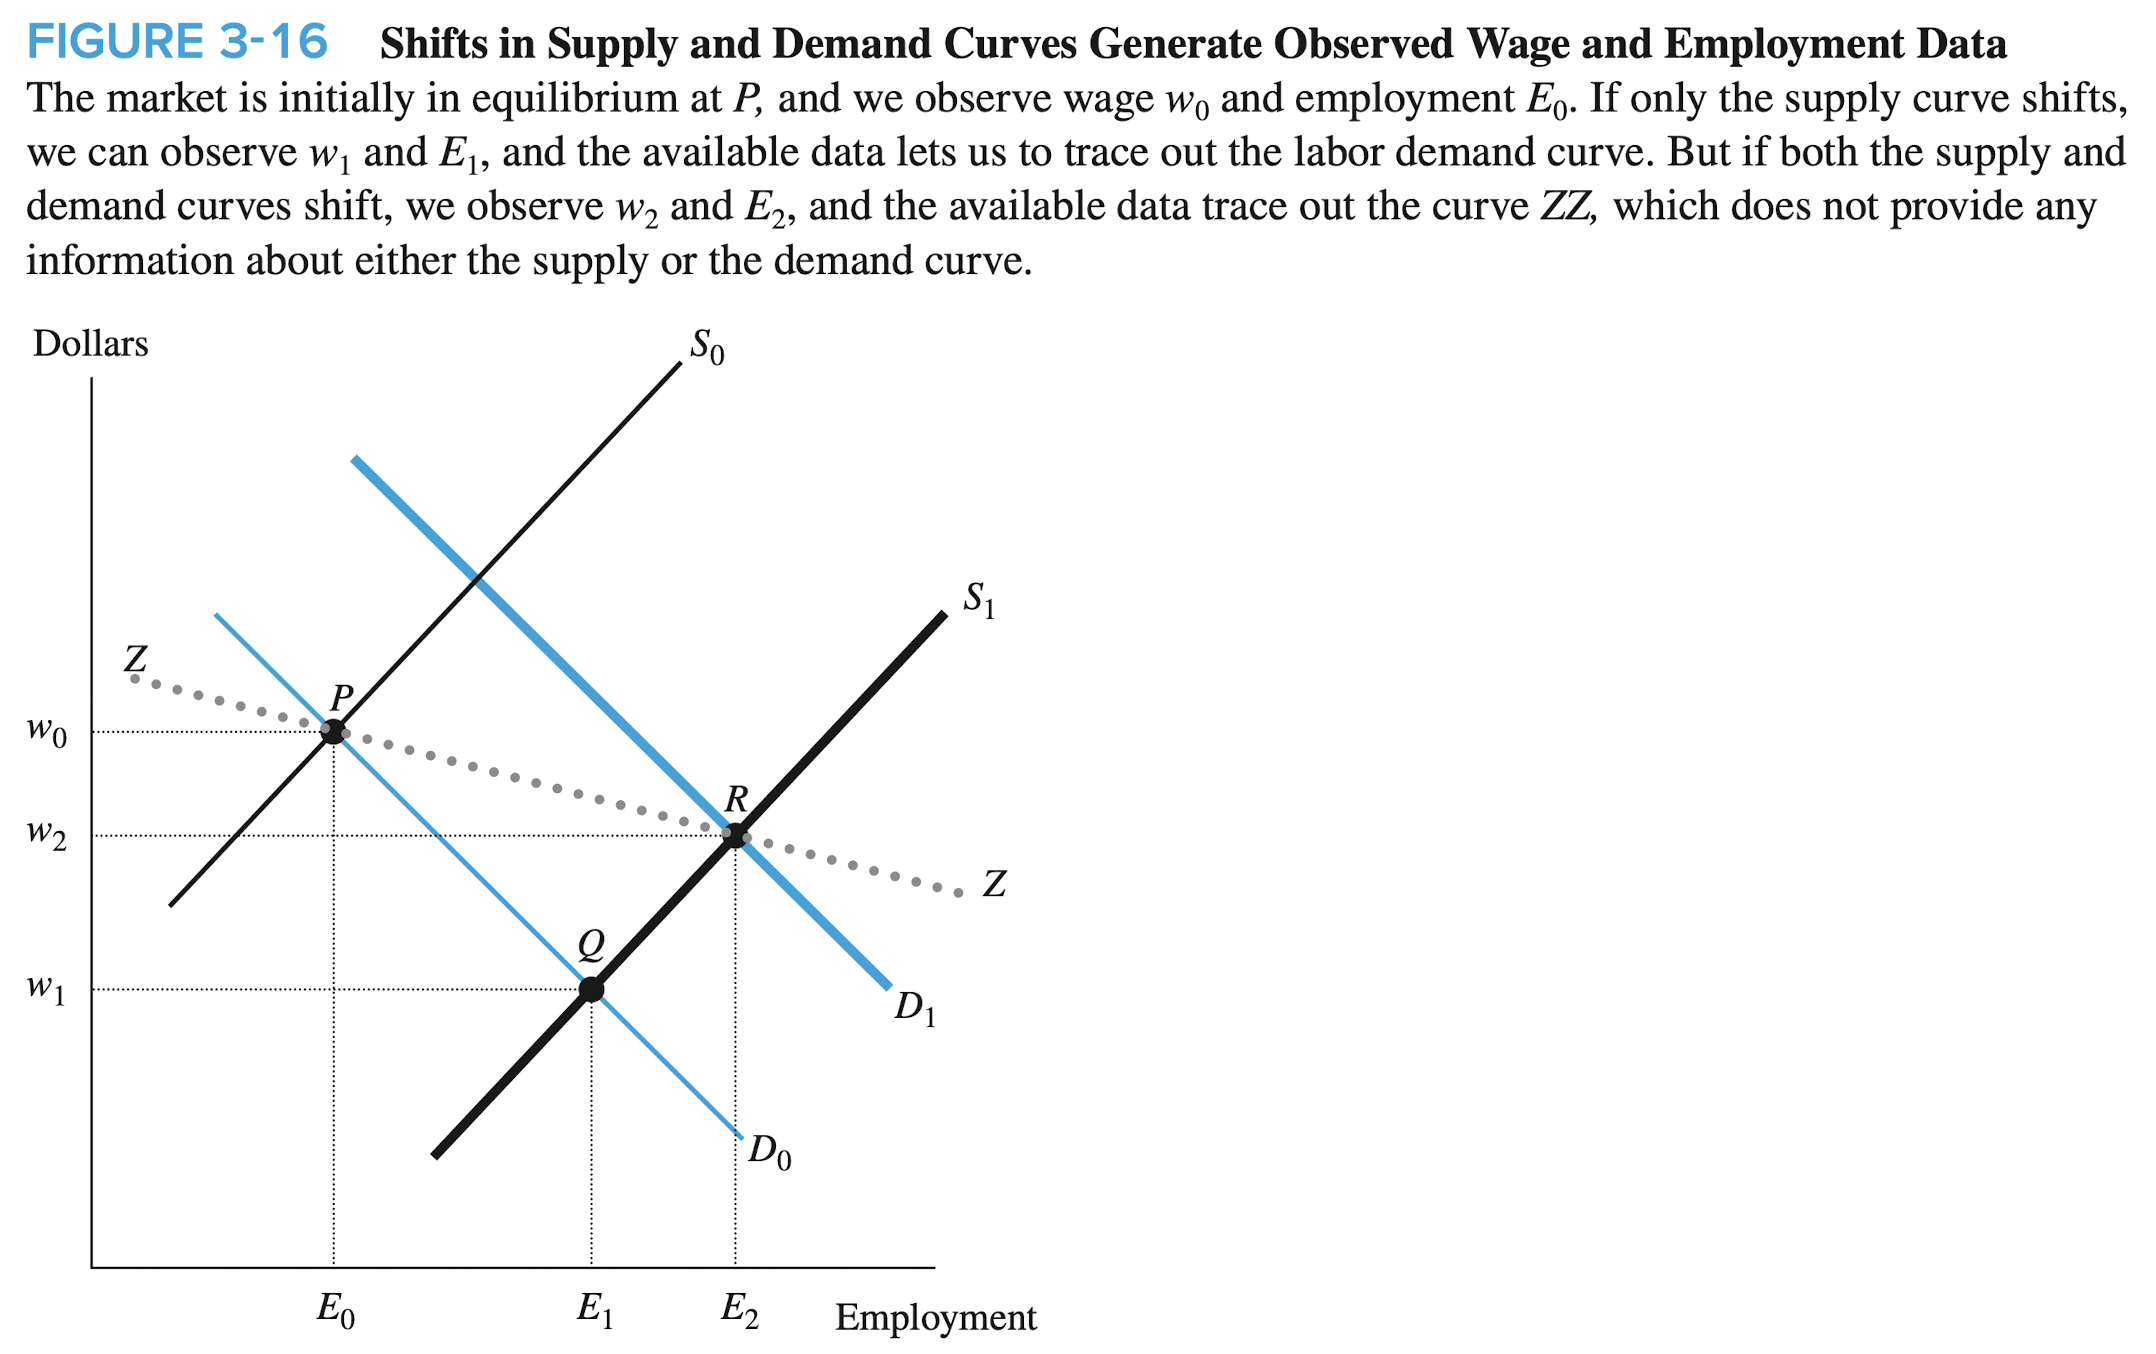
\includegraphics[width=0.95\textwidth]{../input/ch_3p9_instrument_dem.png}
    \caption{Instrumental Variable Approach}
    \label{fig:ch_3p9_instrument_dem}
\end{figure}

\FloatBarrier

The author then describes one paper 
that uses this approach in the context of 
WWII, in which geographic differences in the 
mobilization rate of men was used as 
an instrument for female labor supply.

%%%%%%%%%%%%%%%%%%%%%%%%%%%%%%%%%%%%%%%%%%%%%%%%%%%%%%%%%%%%%%%%%%%%%%%%%%%%%%%%%%%%%%%
%%%%%%%%%%%%%%%%%%%%%%%%%%%%%%%%%%%%%%%%%%%%%%%%%%%%%%%%%%%%%%%%%%%%%%%%%%%%%%%%%%%%%%%
\subsection{Policy Application: The Minimum Wage}

We start by studying the effect of the 
minimum wage in a perfectly competitive labor market;
we will discuss its effects under monospony in a future 
chapter.
\autoref{fig:ch_3p10_min_wage_effect}
will be our reference point for this discussion. 
Prior to the minimum wage, 
the labor market is in equilibrium at
$(E^*, w^*)$. Then, suppose that a minimum wage
is imposed at $\bar{w}$. Now, the labor supply is 
$E_S$, while the labor demand is 
$\bar{E}$. Thus, there are 
$E^* - \bar{E}$ fewer workers employed,
and $E_S - E^*$ workers who want to work
but cannot find jobs (i.e., who are ``unemployed''). 

\FloatBarrier

\begin{figure}[!htb]
    \centering
        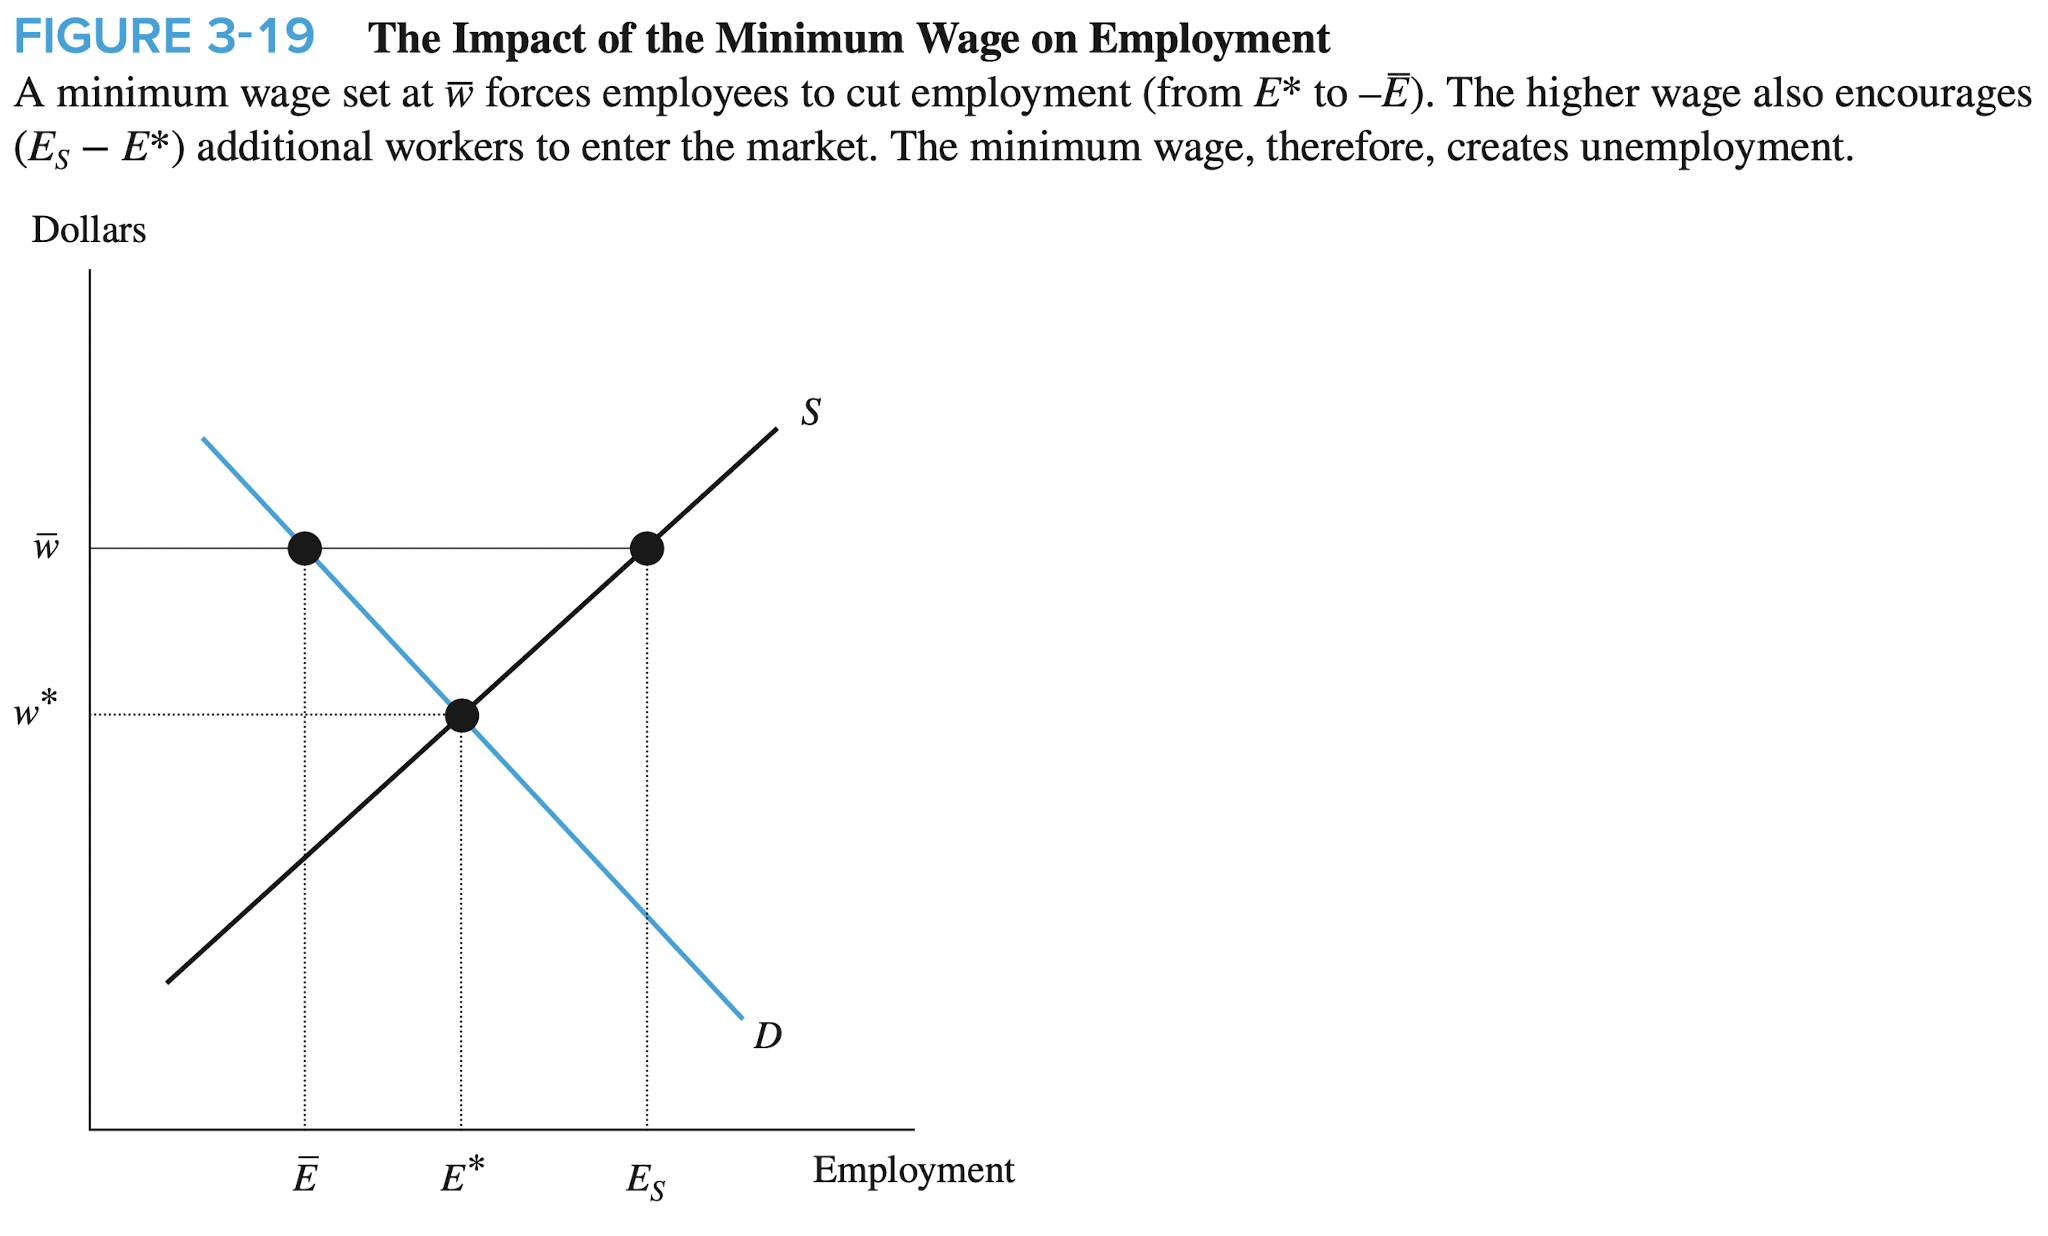
\includegraphics[width=0.95\textwidth]{../input/ch_3p10_min_wage_effect.png}
    \caption{Minimum Wage Effects}
    \label{fig:ch_3p10_min_wage_effect}
\end{figure}

\FloatBarrier

The author then discusses 
compliance with minimum wage and how it 
relates to covered and uncovered sectors, but I won't 
discuss these here at the moment.
The author then gives a lengthy discussion of 
the evidence and debates 
surrounding the effect of the minimum wage on employment.
Again, I will not 
relay it all here, but it's available in the book 
for review.